\chapter{$SO(3)$: The Rotation Group in Three Dimensions}\label{so3}

Similar to $SO(2)$, the group $SO(3)$ represents all possible ways to take the physical action of rotating a vector in space. However, the space we can rotate within has changed to a three-dimensional space for this group, allowing us to have far more possibilities for our rotations. While we will make some simplifying generalizations here, this group still becomes incredibly more complicated than its two-dimensional counterpart. We will assume all rotations take place in $\R^3$. Like before, we will always assume our angle of rotation is real-valued, but we do not specify yet an orientation about which positive rotation occurs. Unless otherwise indicated, we will take $\{e_1,e_2,e_3\}$ to be an orthonormal basis of $\R^3$. This chapter follows the structure laid out in Wu-ki Tung's \textit{Group Theory in Physics}. \cite{Tung}

\section{Construction and Properties}

If we define $SO(3)$ to act on $\R^3$ in a similar way that $SO(2)$ acts on $\R^2$, we could not as easily uncover a formulation for every matrix. Instead, we use the characteristics of $SO(2)$ to guide our intuition for a way to understand the matrices that compose $SO(3)$. Firstly, any rotation should leave the magnitude of a vector in $\R^3$ unchanged. This leads us to conclude that the matrices must be orthogonal. Further, it will also follow that these matrices have determinant $1$, since all rotations can be reached continuously from the identity. With this information alone, we can deduce that the $SO(3)$ matrices form a group under matrix multiplication. The question of classifying these matrices is still open for us to answer. There are two main ways we can do so.

In two dimensions, it is straightforward to define a convention for orientation and measurement of any rotation. However, when we get to three dimensions, we need to be more careful about how we describe these actions. Our first attempt to characterize these will have us focus on embedding two-dimensional rotations in three-dimensional space. First, let us consider any $n\in\R^3$. We can treat this vector as an axis about which we rotate by taking the plane normal to it. Once we have rotated vectors about this axis, we can measure the angle of rotation by projecting these vectors onto the normal plane and calculating the angle just as we did in our two-dimensional derivation in Chapter 2. We still take the convention that positive angle measurements correspond to a counter-clockwise rotation about in the normal plane. The orientation of $n$ is uniquely determined by two angles, $\theta$ and $\phi$, as defined by spherical coordinates in $\R^3$. For this discussion, we do not care about $||n||$, since this value does not impact the direction the axis points. In this way, every possible rotation in $\R^3$ is characterized by one angle of counter-clockwise rotation and the two angles that determine the orientation about which we rotate (the direction that $n$ points). In other words, the rotation, which we will refer to as $R_n(\psi) = R_{\theta,\phi}(\psi)$, identifies a rotation as displayed in the picture below.


\begin{figure}{H}
	\centering
	\tdplotsetmaincoords{60}{120}
	\tdplotsetrotatedcoords{60}{45}{225}
	\centering
	\begin{tikzpicture}
			[scale=1.2,
				tdplot_main_coords,
				axis/.style={->,black,thin},
				vector/.style={-stealth,black,very thick}]
	

		%draw the axes
		\draw[axis] (0,0,0) -- (3,0,0) node[anchor=west]{$x$};
		\draw[axis] (0,0,0) -- (0,3,0) node[anchor=west]{$y$};
		\draw[axis] (0,0,0) -- (0,0,3) node[anchor=west]{$z$};
	
		\coordinate (O) at (0,0,0);
		\tdplotsetcoord{P}{3}{45}{60}

	%	\draw[thick,tdplot_rotated_coords,->](0,0,0)--(.5,0,0)node[anchor=west]{$x'$};
		%\draw[thick,tdplot_rotated_coords,->](0,0,0)--(0,.5,0)node[anchor=west]{$y'$};
		%\draw[thick,tdplot_rotated_coords,->](0,0,0)--(0,0,5)node[anchor=west]{$z'$};
		\draw[dashed,color=red] (O)--(Pxy);
		\draw[dashed,color=red] (P)--(Pxy);
		%x =  y = z=2.09 r = 2.15218
	\tdplotsetrotatedcoords{60}{45}{225}
		\tdplotdrawarc[->,tdplot_rotated_coords,color=blue, very thick]{(0,0,0)}{0.5}{0}{360}{anchor=south west}{$\psi$};
		\tdplotdrawarc[->]{(0,0,0)}{2.15218}{0}{60}{anchor=north}{$\theta$};
		\tdplotsetrotatedcoords{-30}{-90}{0}
		\tdplotdrawarc[->,tdplot_rotated_coords]{(0,0,0)}{2}{0}{45}{anchor=north east}{$\phi$};
		\draw[->, very thick] (O) -- (P) node[anchor=south]{$n$} ;			
	\end{tikzpicture}
	\caption{Generic rotation in $SO(3)$ characterized by $R_n(\psi)$}		
\end{figure}

By identifying rotations with these three parameters, we create some redundancy. Specifically, for any direction, $n$, the following equality holds:

$$R_n(\psi) = R_{-n}(2\pi - \psi)$$

\noindent as evidenced by the following picture: 

\begin{figure}[H]
	\begin{tabular}{ccccc}
		\tdplotsetmaincoords{60}{120}
	
				\begin{tikzpicture}
						[scale=1,
							tdplot_main_coords,
							axis/.style={->,black,thin},
							vector/.style={-stealth,black,very thick}]
				
				
					\coordinate (O) at (0,0,0);
					\coordinate (r1) at (1.414,0,1);
					\coordinate (r2) at (0,-1.414,1);
					\coordinate (r3) at (-1.414,-0,1);
					\coordinate (r4) at (0,1.414,1);
					\coordinate (r5) at (1.414,0,-1);
					\coordinate (r6) at (0,-1.414,-1);
					\coordinate (r7) at (-1.414,0,-1);
					\coordinate (r8) at (0,1.414,-1);
		
		
					\draw[axis,color=gray] (0,0,0) -- (0,0,-2) node[anchor=west]{$-n$};
					
					\draw[color=gray] (r1)--(r2);
					\draw[color=gray] (r2)--(r3);
					\draw[color=gray] (r3)--(r4);
					\draw[color=gray] (r4)--(r1);
					\draw[color=gray] (r1)--(r5);
					\draw[color=gray] (r2)--(r6);
					\draw[color=gray] (r3)--(r7);
					\draw[color=gray] (r4)--(r8);
					\draw[color=gray] (r5)--(r6);
					\draw[color=gray] (r6)--(r7);
					\draw[color=gray] (r7)--(r8);
					\draw[color=gray] (r8)--(r5);
		
					
		
				\end{tikzpicture}
		&
	\begin{LARGE}
	$\overset{R_{-n}(2\pi-\psi)}{\leftarrow}$
	\end{LARGE}
	&
	\tdplotsetmaincoords{60}{120}
		%\tdplotsetrotatedcoords{60}{45}{225}
				\begin{tikzpicture}
						[scale=1,
							tdplot_main_coords,
							axis/.style={->,black,thin},
							vector/.style={-stealth,black,very thick}]
				
				
					\coordinate (O) at (0,0,0);
					\coordinate (r1) at (1,1,1);
					\coordinate (r2) at (-1,1,1);
					\coordinate (r3) at (-1,-1,1);
					\coordinate (r4) at (1,-1,1);
					\coordinate (r5) at (1,1,-1);
					\coordinate (r6) at (-1,1,-1);
					\coordinate (r7) at (-1,-1,-1);
					\coordinate (r8) at (1,-1,-1);
		
		
					\draw[axis,color=black] (0,0,0) -- (0,0,2) node[anchor=west]{$n$};
					\draw[axis,color=gray] (0,0,0) -- (0,0,-2) node[anchor=west]{$-n$};
					\draw[color=gray] (r1)--(r2);
					\draw[color=gray] (r2)--(r3);
					\draw[color=gray] (r3)--(r4);
					\draw[color=gray] (r4)--(r1);
					\draw[color=gray] (r1)--(r5);
					\draw[color=gray] (r2)--(r6);
					\draw[color=gray] (r3)--(r7);
					\draw[color=gray] (r4)--(r8);
					\draw[color=gray] (r5)--(r6);
					\draw[color=gray] (r6)--(r7);
					\draw[color=gray] (r7)--(r8);
					\draw[color=gray] (r8)--(r5);
	
					\tdplotsetrotatedcoords{225}{180}{0}
	
					\coordinate (Shift1) at (0,0,1);
					\tdplotsetrotatedcoordsorigin{(Shift1)};
					\tdplotdrawarc[->,tdplot_rotated_coords,color= blue, thick]{(0,0,0)}{1.414}{0}{45}{anchor=south}{$\psi$};
	
					\coordinate (Shift2) at (0,0,-1);
					\tdplotsetrotatedcoordsorigin{(Shift2)};
					\tdplotdrawarc[->,tdplot_rotated_coords,color= bluegray, thick]{(0,0,0)}{1.414}{0}{-315}{anchor=north}{$2\pi-\psi$};
					\draw[dashed, color=black] (1.414,0,-1.5) -- (1.414,0,2);
		
	
					
		
				\end{tikzpicture}	
	
	
	&
	\begin{LARGE}
	$\overset{R_n(\psi)}{\rightarrow}$
	\end{LARGE}
	&
	\tdplotsetmaincoords{60}{120}
		%\tdplotsetrotatedcoords{60}{45}{225}
				\begin{tikzpicture}
						[scale=1,
							tdplot_main_coords,
							axis/.style={->,black,thin},
							vector/.style={-stealth,black,very thick}]
				
				
					\coordinate (O) at (0,0,0);
					\coordinate (r1) at (1.414,0,1);
					\coordinate (r2) at (0,-1.414,1);
					\coordinate (r3) at (-1.414,-0,1);
					\coordinate (r4) at (0,1.414,1);
					\coordinate (r5) at (1.414,0,-1);
					\coordinate (r6) at (0,-1.414,-1);
					\coordinate (r7) at (-1.414,0,-1);
					\coordinate (r8) at (0,1.414,-1);
		
		
					\draw[axis,color=black] (0,0,0) -- (0,0,2) node[anchor=west]{$n$};
					\draw[color=gray] (r1)--(r2);
					\draw[color=gray] (r2)--(r3);
					\draw[color=gray] (r3)--(r4);
					\draw[color=gray] (r4)--(r1);
					\draw[color=gray] (r1)--(r5);
					\draw[color=gray] (r2)--(r6);
					\draw[color=gray] (r3)--(r7);
					\draw[color=gray] (r4)--(r8);
					\draw[color=gray] (r5)--(r6);
					\draw[color=gray] (r6)--(r7);
					\draw[color=gray] (r7)--(r8);
					\draw[color=gray] (r8)--(r5);
		
					
		
				\end{tikzpicture}
	
	
	\end{tabular}
	\caption{Identifying equivalent rotations about vectors pointing in opposite directions.}
\end{figure}

This is truly a consequence of the fact that positive (counter-clockwise) rotation is relative to the direction one faces. Consider placing yourself in the center of the square at the point where $n$ and $-n$ touch. Looking both up and down will show that the angle of rotation is in the counter-clockwise direction. We can match every rotation in one direction with an opposite-direction rotation by another angle using this relationship. In order to keep ourselves from double-counting, we can restrict the values of our parameters to conform to the following convention: 

$$0\leq\psi\leq\pi, \hspace{3mm} 0\leq\theta\leq2\pi, \hspace{3mm} 0\leq\phi\leq\pi$$

While we still have the $\psi=\pi$ case to worry about, this greatly limits the amount of rotations we double-count and is a satisfactory convention. A useful way to visualize each rotation is to view it as a point in $\R^3$ as an ordered triple in spherical coordinates $(\psi,\phi,\theta)$. $\phi$ and $\theta$ are defined conventionally as they are, but $\psi$ takes the place of the value for the distance from the origin. In this way, we identify every point in the sphere of radius $\pi$ centered at the origin with a rotation in $\R^3$ \\

\begin{figure}[H]
	\centering
	\tdplotsetmaincoords{60}{120}
	%\tdplotsetrotatedcoords{60}{45}{225}
	\begin{tikzpicture}
			[scale=2,
				tdplot_main_coords,
				axis/.style={->,black,thin},
				vector/.style={-stealth,black,very thick}]
		\draw[axis,color=gray] (0,0,0) -- (2,0,0) node[anchor=south]{$x$};
		\draw[axis,color=gray] (0,0,0) -- (0,2,0) node[anchor=west]{$y$};
		\draw[axis] (0,0,0) -- (0,0,2) node[anchor=east]{$z$};
		\shade[ball color = gray, opacity=0.5] (0,0,0) circle (0.75cm);
		\draw[->,thick,color=black] (0,0,0) -- (1.8137,1.8137,1.8137) node[anchor=south west]{$R_n(\pi)$};
	
	\end{tikzpicture}
	\caption{Visualization of the group $SO(3)$}
	

\end{figure}

We can use the geometry of three-dimensional space to observe a very simple but powerful fact.

\begin{theorem}
	Let $n, n'\in\R^3$ and $\psi\in[0,\pi]$. Let $R\in SO(3)$ be a rotation that takes $n$ and points it in the direction of $n'$. Then, the following identity holds:
$$R_{n}(\psi) = R^{-1}R_{n'}(\psi)R$$
\end{theorem}

This identity can be easily verified as seen in the following sequence of images\\

\begin{figure}[H]
	\centering
	\begin{tabular}{cc}
		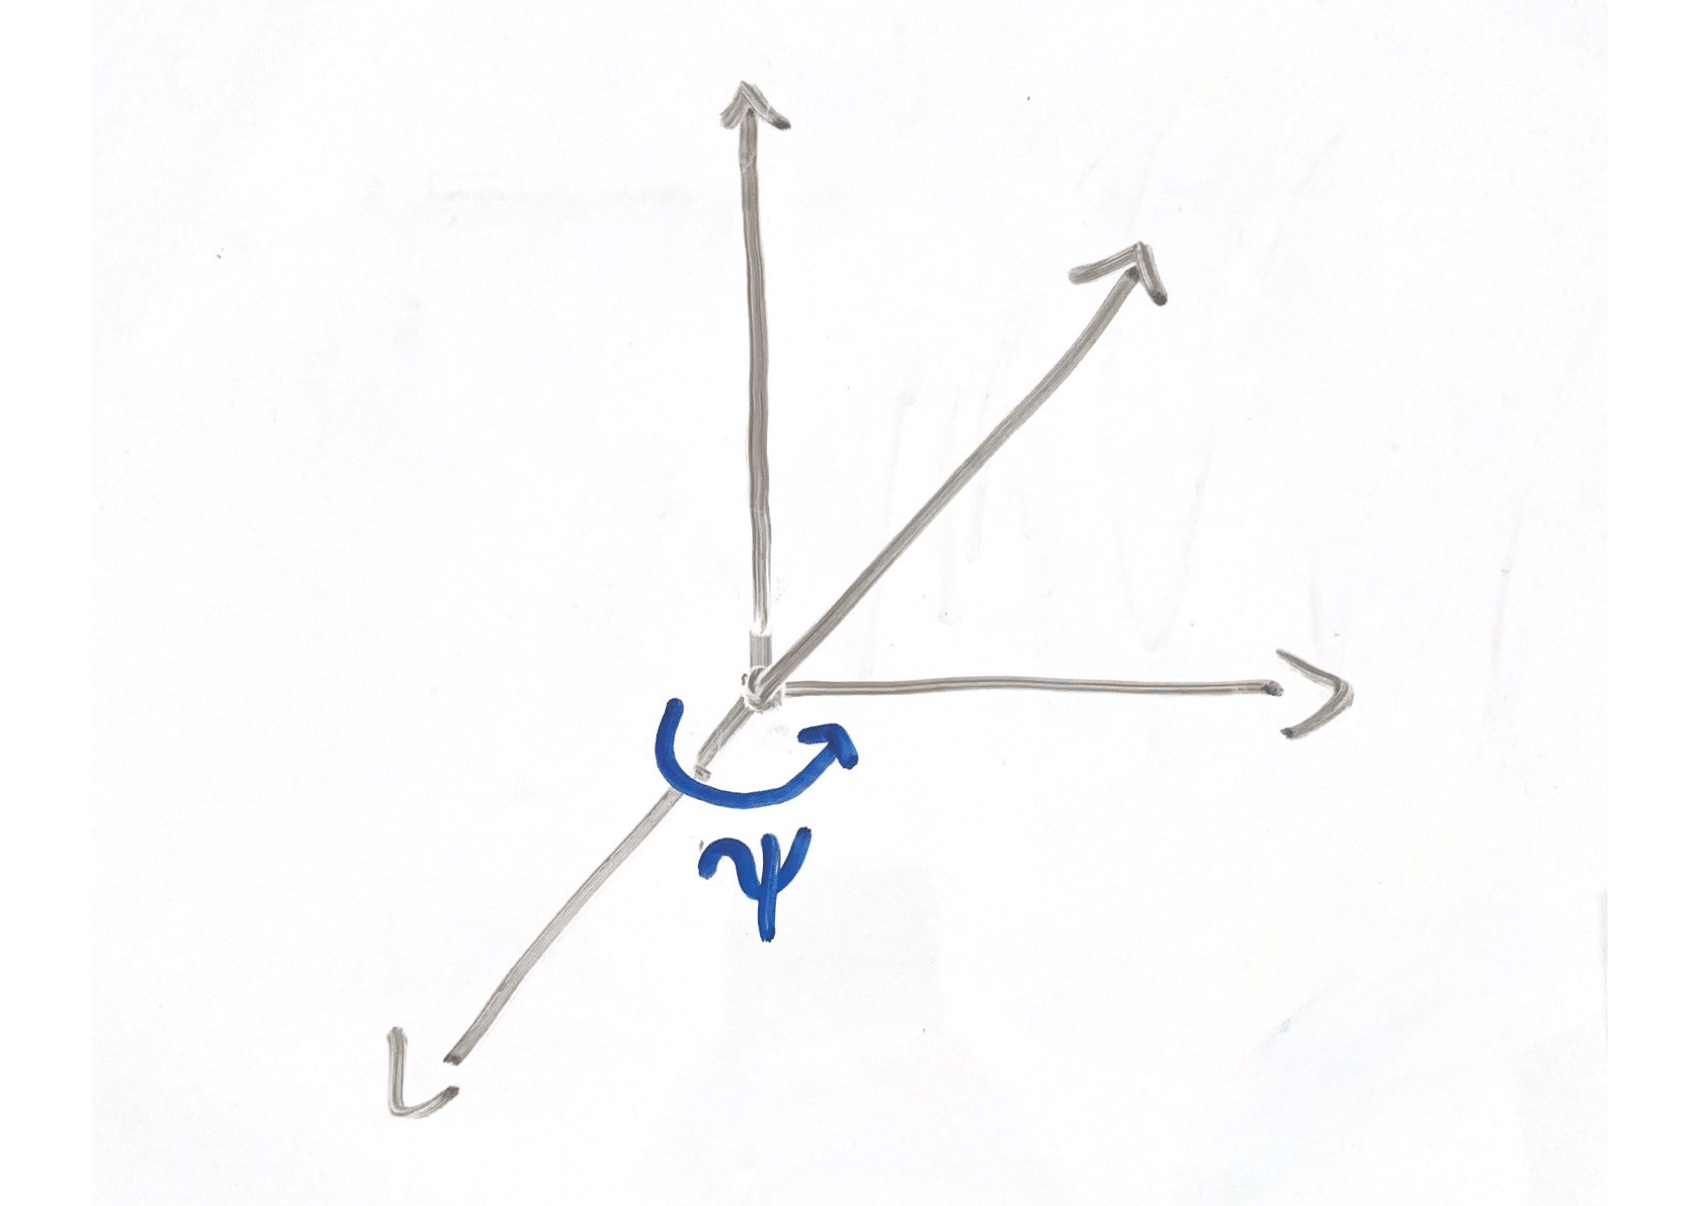
\includegraphics[width=0.4\textwidth]{Rnpsi1.png}
&
		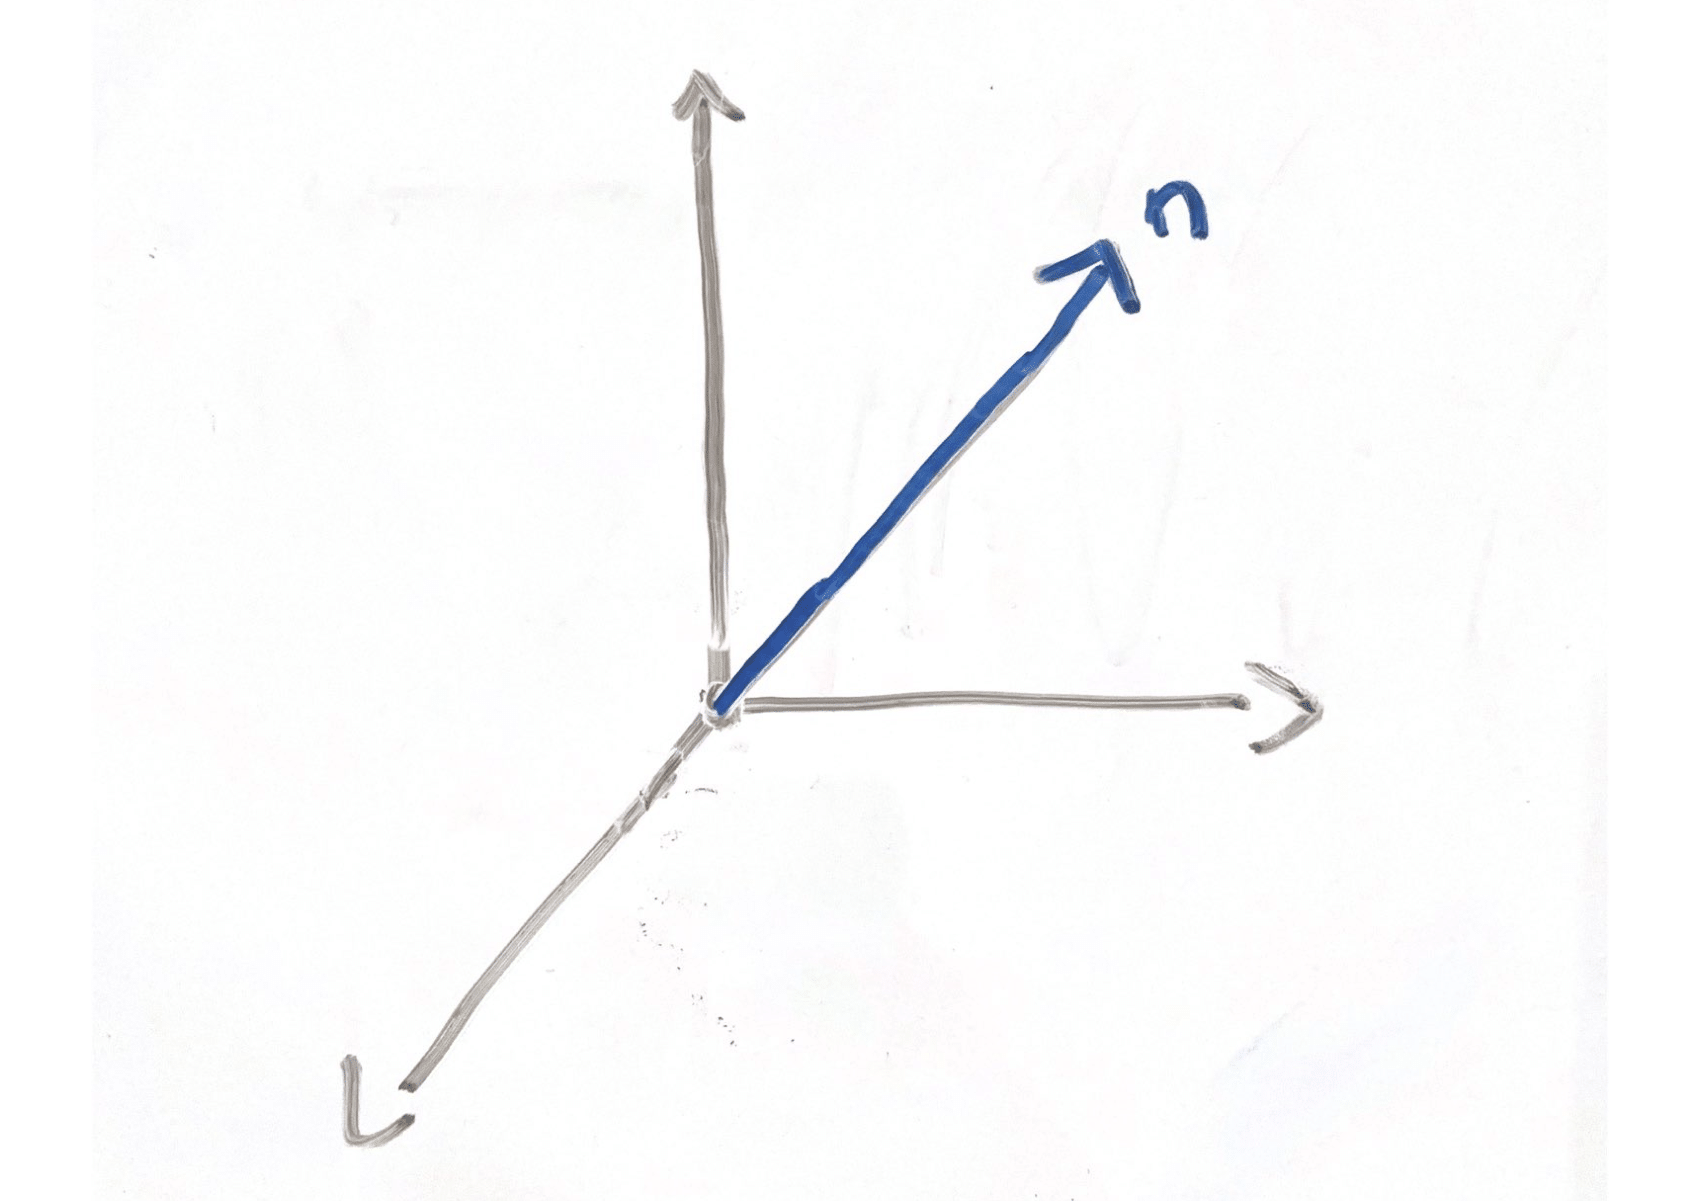
\includegraphics[width=0.4\textwidth]{Rnpsi2.png}
	\end{tabular}
	\caption{Theorem 3.1: $R_n(\psi)$}
	

\end{figure}
\begin{figure}[H]
	\centering

	\begin{tabular}{ccc}
		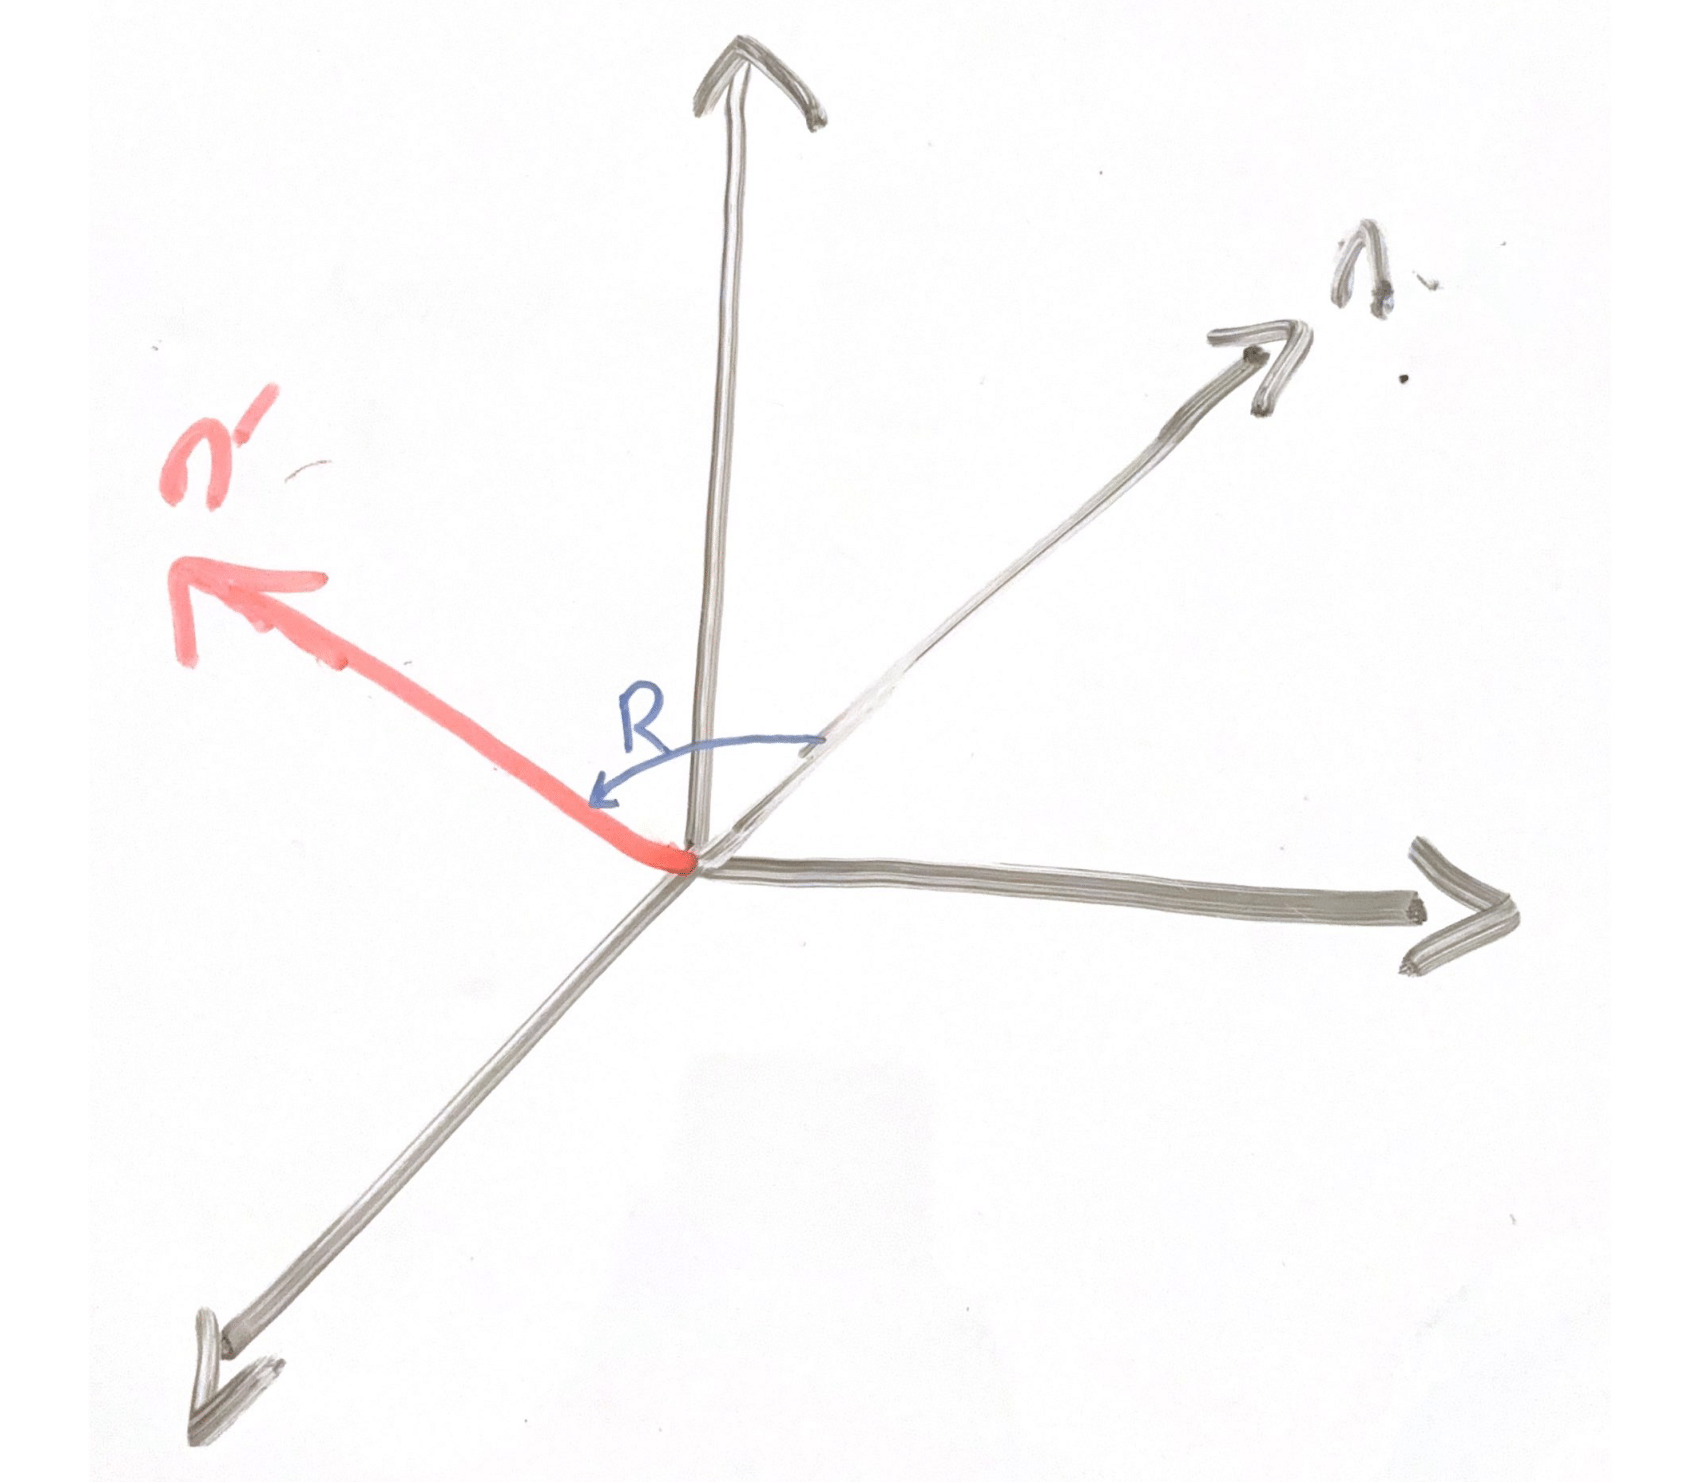
\includegraphics[width=0.3\textwidth]{RRnR1.png}
		&
		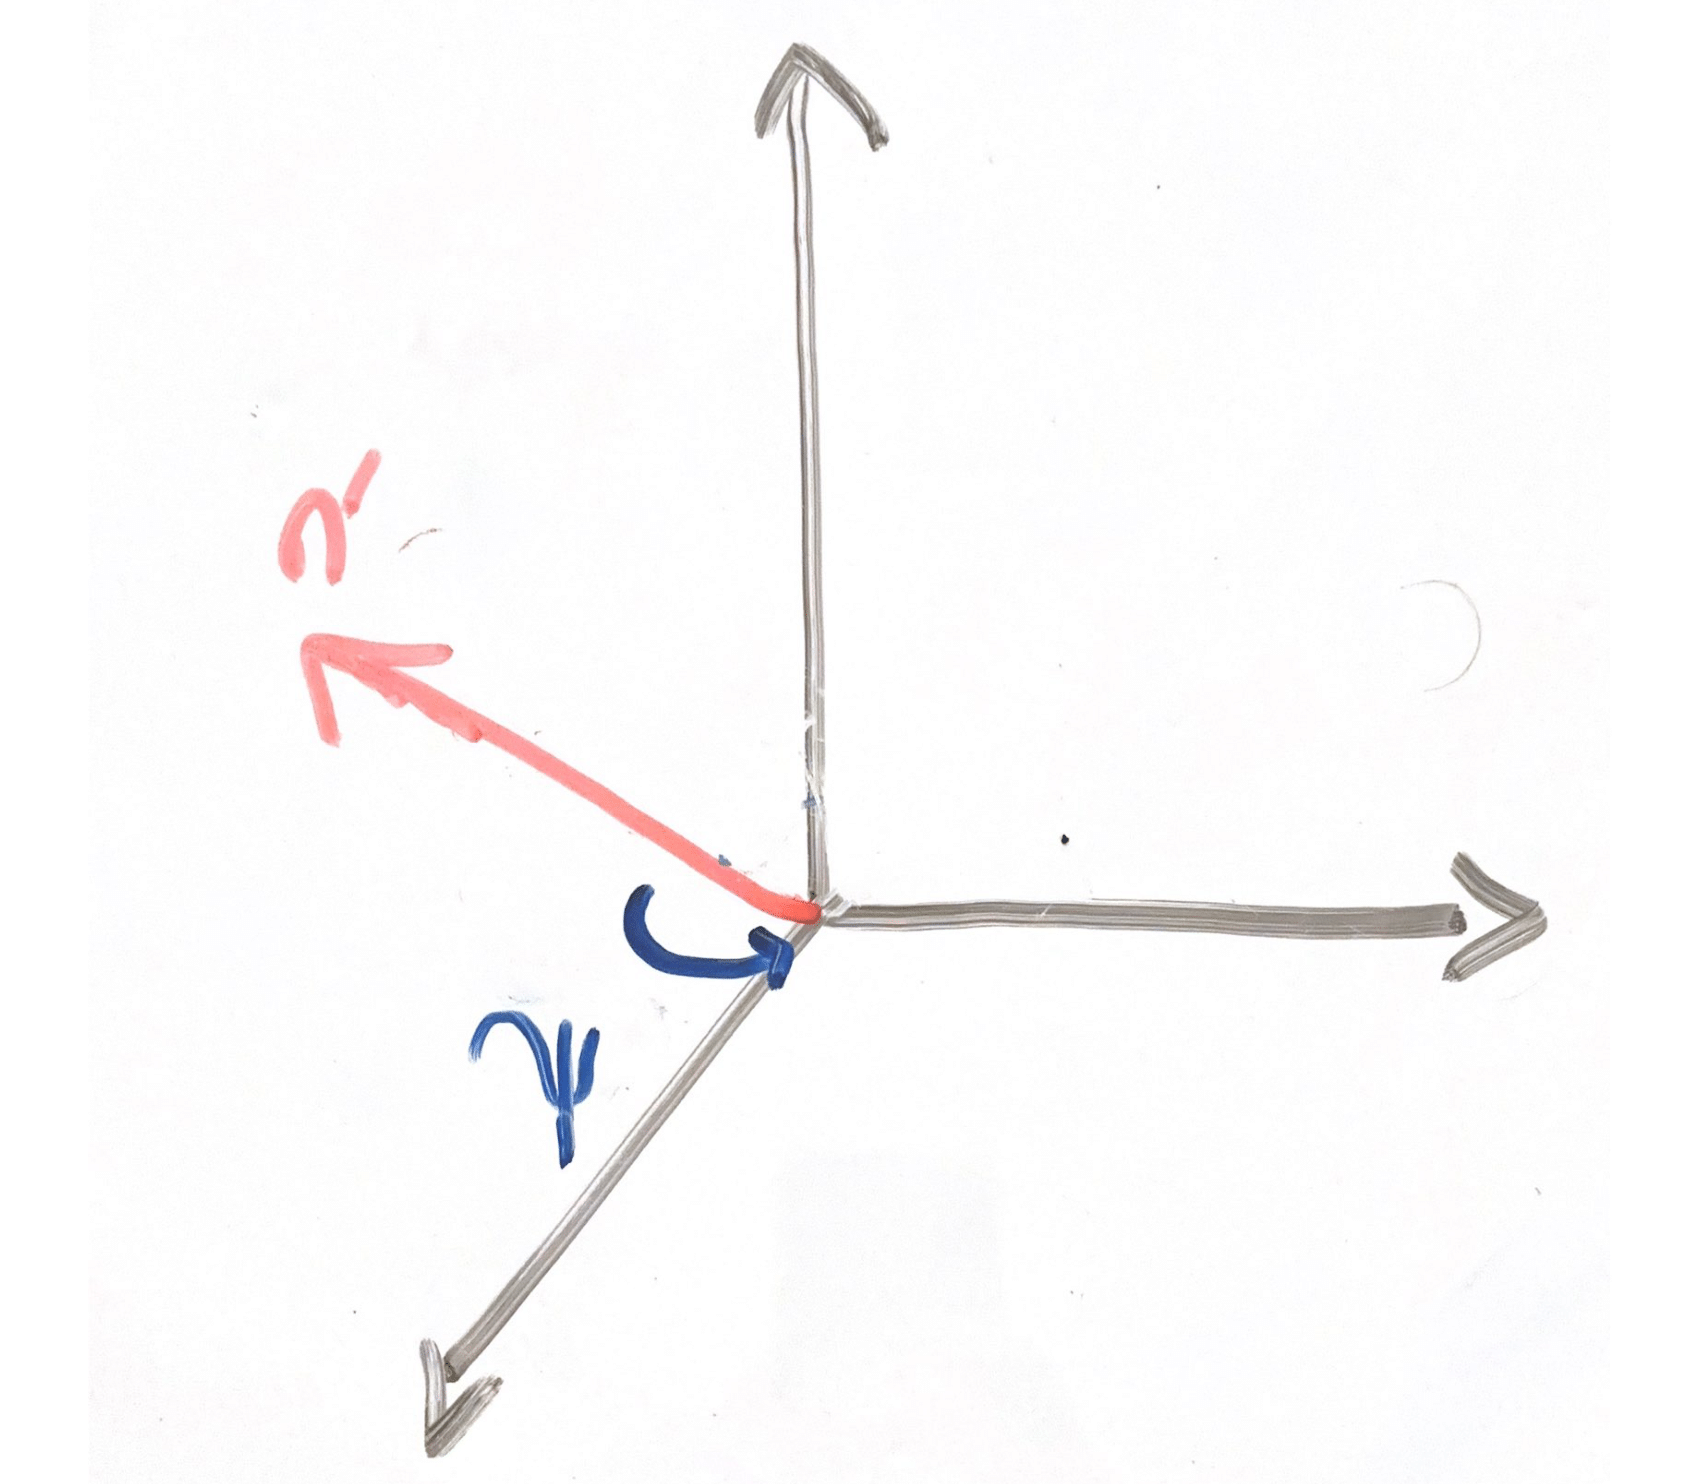
\includegraphics[width=0.3\textwidth]{RRnR2.png}\\
		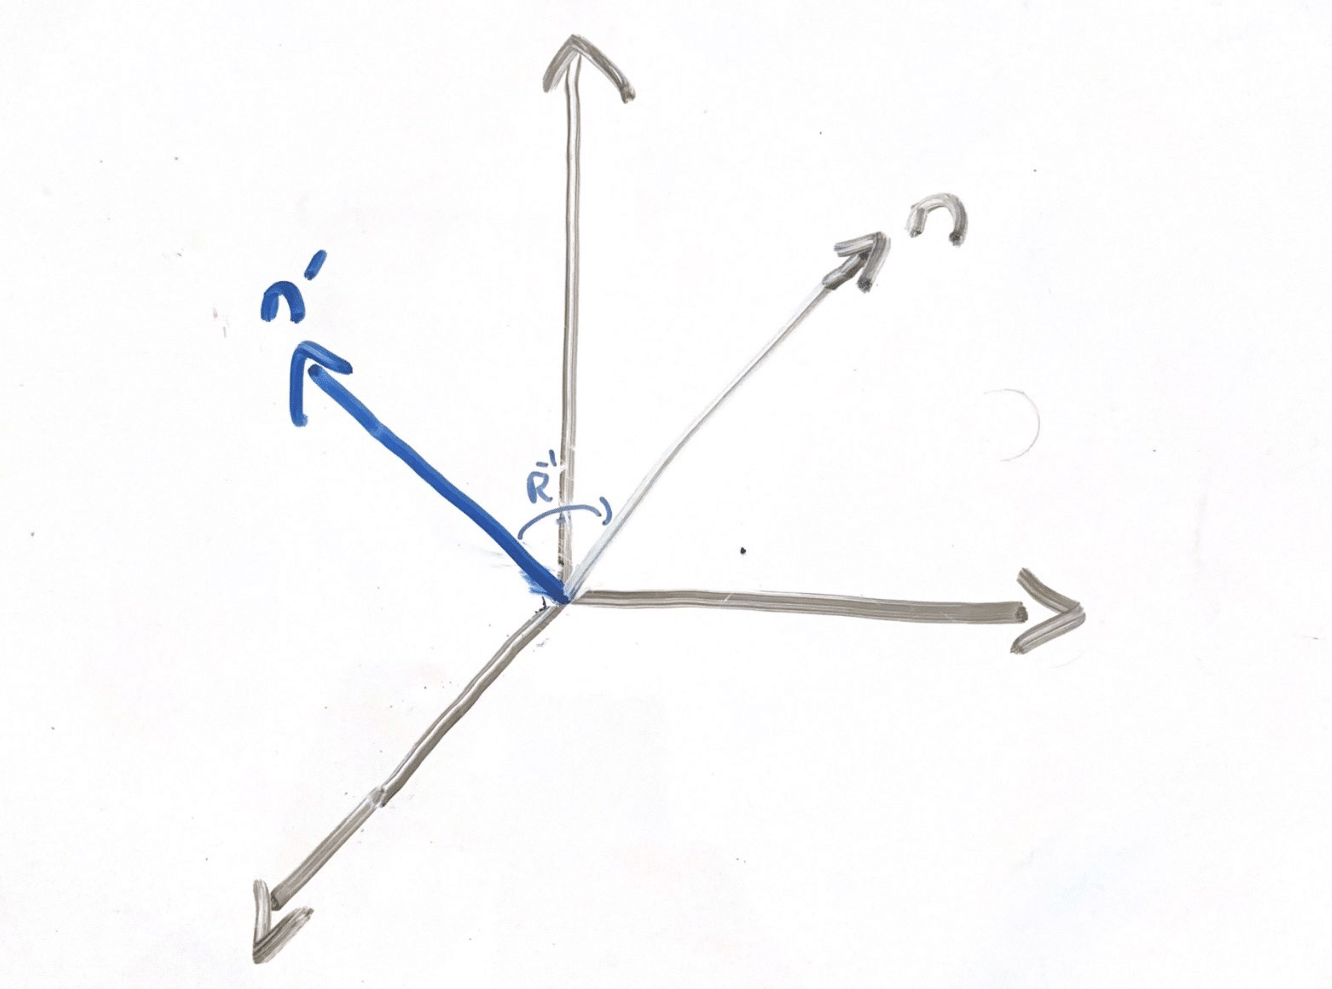
\includegraphics[width=0.3\textwidth]{RRnR3.png}
		&
		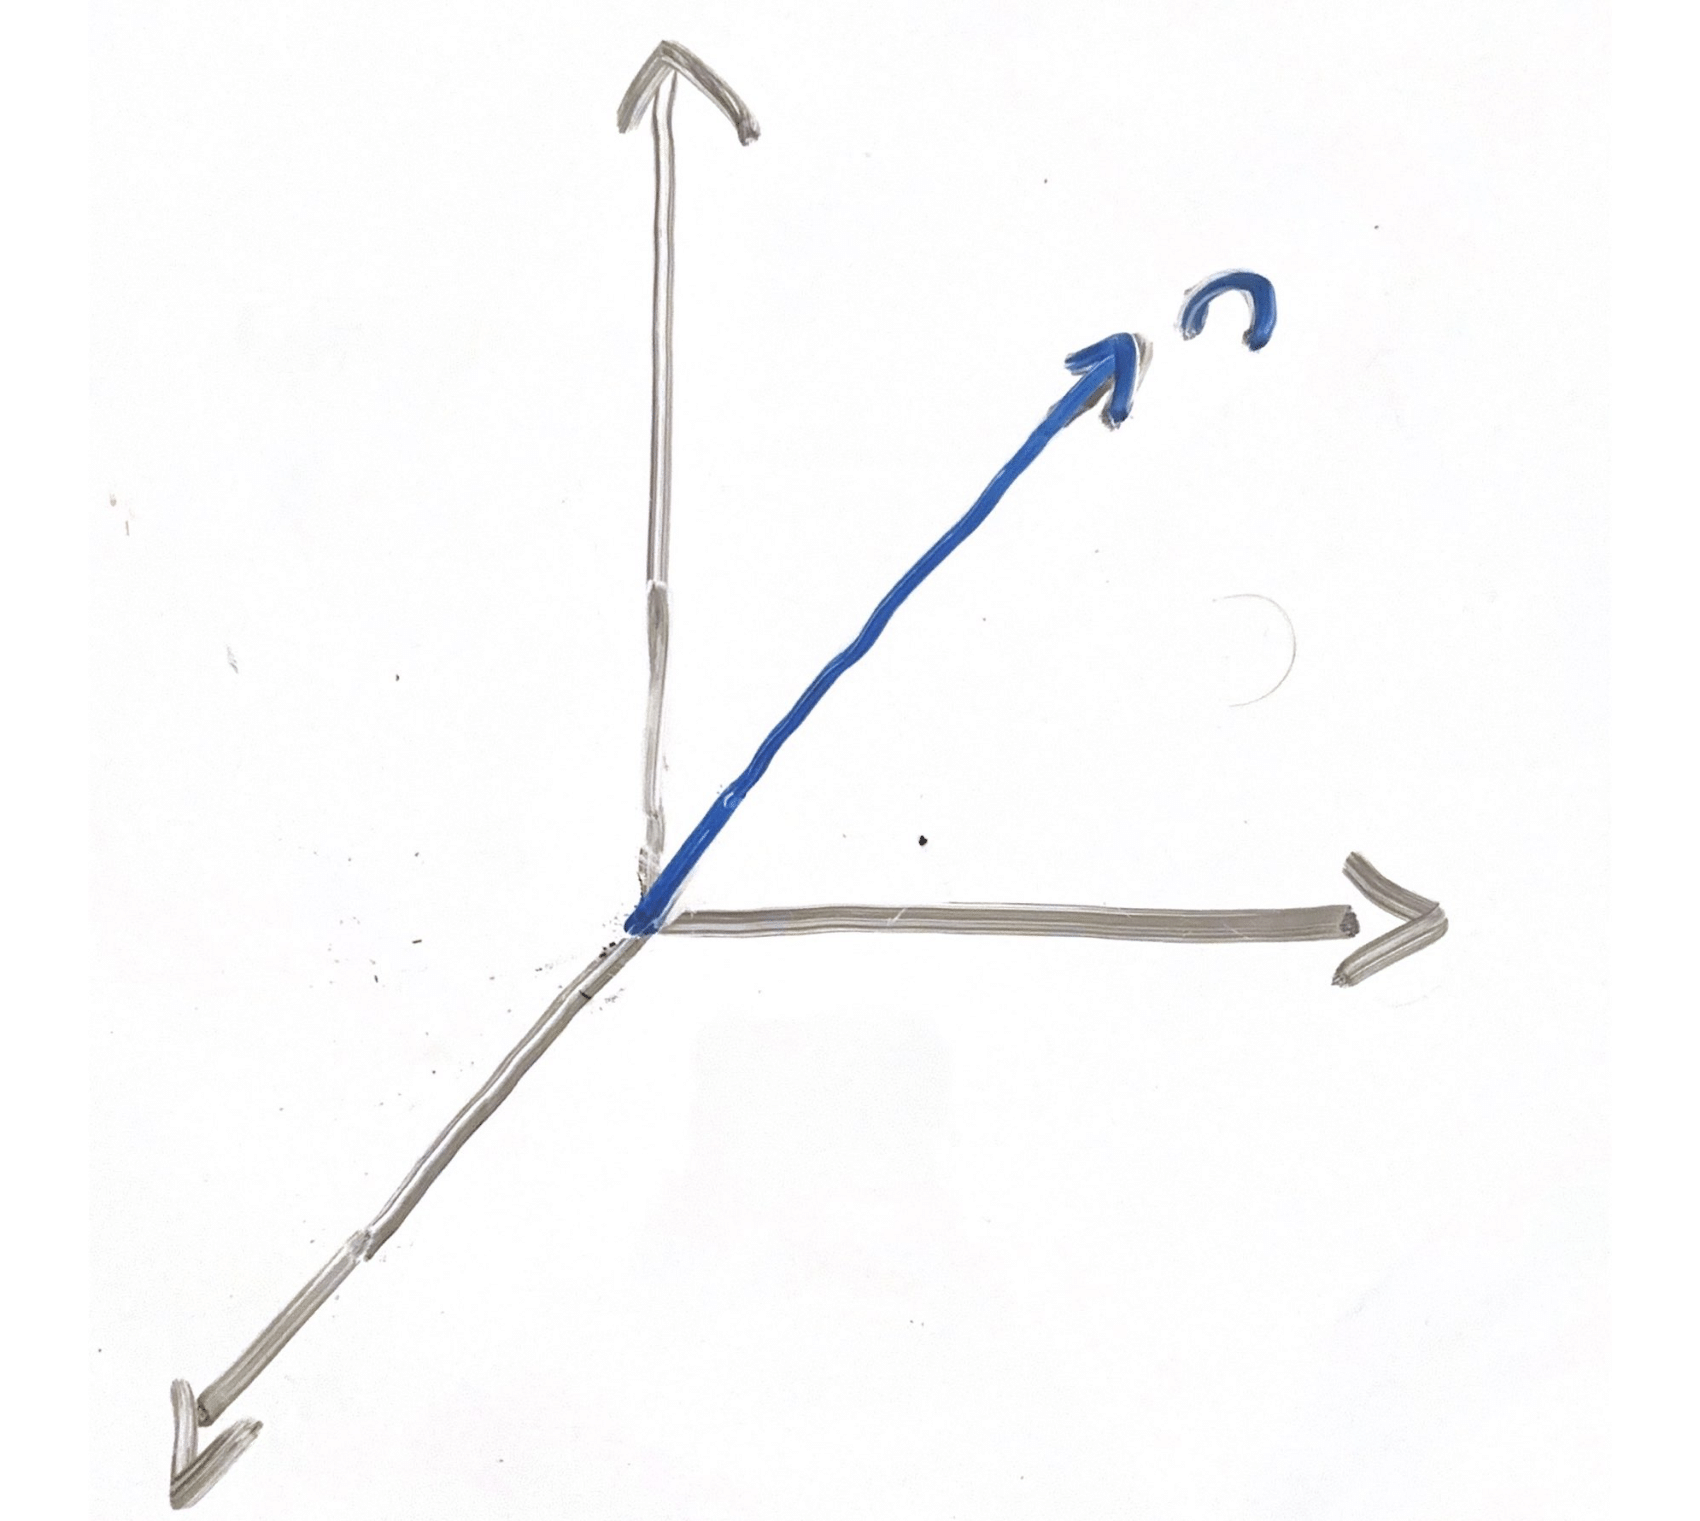
\includegraphics[width=0.3\textwidth]{RRnR4.png}

	\end{tabular}
	\caption{Theorem 3.1: $R^{-1}R_{n'}(\psi)R$}
	

\end{figure}



With this identity in mind, we can make a deeper conclusion about the inherent structure of $SO(3)$.

\begin{corrolary}
	All rotations (about any axis) by a fixed angle $\psi$ share a conjugacy class (denoted $C_\psi$).
\end{corrolary}

These classifications of rotations give us our first way of understanding rotations in $SO(3)$. There is another equally useful way to interpret any rotation in $\R^3$. Suppose our coordinate axes are defined by the following convention: $(x,y,z)$. A rotation in $SO(3)$ will change the direction that these axes point in, but still will preserve the inherent mutual orthogonality of the directions. We will refer to the initial axes as the "fixed frame" and the rotated axes, $(x',y',z')$, as the rotated frame. The natural question would be to ask how we can characterize the transition from the fixed frame to the rotated frame.

\begin{definition}
	Let $(x,y,z)$ be the fixed frame and let $(x',y',z')$ be any rotated frame. Then this rotation's \textbf{Euler Angles} decompose the rotation in the following way:
$$R(\alpha,\beta,\gamma) \coloneq R_{z'}(\gamma)R_n(\beta)R_z(\alpha)$$
where $n$ points in the direction defined by the intersection of the $xy$ and $x'y'$ planes (or equivalently, the $z\times z'$ direction). Note: we use the subscript $z$ and $z'$ as a shorthand to mean the $z$-axis and $z'$-axis.
\end{definition}

In this way, we view every rotation in $SO(3)$ as the composition of three rotations about mutually orthogonal axes. Conventionally, we restrict the parameters to the following conditions: $\alpha,\gamma\in[0,2\pi)$, $\beta\in[0,\pi]$. This limits double-counting in a similar manner to the discussion above. The figure below illustrates the use of Euler angles to complete an arbitrary rotation as the composition of three determined rotations.\\

\begin{figure}[H]
	\centering
	\tdplotsetmaincoords{60}{200}
	\tdplotsetrotatedcoords{60}{45}{225}
	\begin{tikzpicture}
			[scale=2,
				tdplot_main_coords,
				axis/.style={->,black,thin},
				vector/.style={-stealth,black,very thick}]
		\draw[axis,color=gray] (0,0,0) -- (1,0,0) node[anchor=south]{$x$};
		\draw[axis,color=gray] (0,0,0) -- (0,1,0) node[anchor=west]{$y$};
		\draw[axis] (0,0,0) -- (0,0,1) node[anchor=east]{$z$};
		\draw[axis,color=blue] (0,0,0) -- (-0.707106781186548,0.707106781186548,0) node[anchor=west]{$z'$}; 
		\tdplotcrossprod(-0.707106781186548,0.707106781186548,0)(0,0,1);
		\draw[axis,color=red] (0,0,0)--(\tdplotresx,\tdplotresy,\tdplotresz) node[anchor=south]{$n$};
		\tdplotdrawarc[->]{(0,0,0)}{1.2}{0}{315}{anchor=north}{$\alpha$};
	\end{tikzpicture}
	\caption{Euler Angles: Rotating Fixed Frame about $z$-axis by $\alpha$}
		
\end{figure}

\begin{figure}[H]
	\centering
	\tdplotsetmaincoords{60}{200}
	\tdplotsetrotatedcoords{45}{90}{90}
	\begin{tikzpicture}
			[scale=2,
				tdplot_main_coords,
				axis/.style={->,black,thin},
				vector/.style={-stealth,black,very thick}]
		\draw[axis,color=lightgray] (0,0,0) -- (1,0,0) node[anchor=south]{$x$};
		\draw[axis,color=black] (0,0,0) -- (0.7071,-0.7071,0) node[anchor=north]{$x$};
		\draw[axis,color=lightgray] (0,0,0) -- (0,1,0) node[anchor=west]{$y$};
		\draw[axis,color=black] (0,0,0) -- (0,0,1) node[anchor=east]{$z$};
		\draw[axis,color=blue] (0,0,0) -- (-0.707106781186548,0.707106781186548,0) node[anchor=east]{$z'$};
		\tdplotcrossprod(-0.707106781186548,0.707106781186548,0)(0,0,1);
		\draw[axis,color=wildwatermelon] (0,0,0)--(\tdplotresx,\tdplotresy,\tdplotresz) node[anchor=south]{$y$};
		\tdplotdrawarc[->,color=gray]{(0,0,0)}{1.2}{0}{315}{anchor=south east}{$\alpha$};
		\tdplotdrawarc[<-,tdplot_rotated_coords,color=red]{(0,0,0)}{1.2}{0}{90}{anchor=south west}{$\beta$};
	\end{tikzpicture} 
	\caption{Euler Angles: Rotating Intermediate Frame about new $y$-axis by $\beta$}
\end{figure}

\begin{figure}[H]
	\centering
	\tdplotsetmaincoords{60}{200}
	\tdplotsetrotatedcoords{45}{90}{90}
	\begin{tikzpicture}
			[scale=2,
				tdplot_main_coords,
				axis/.style={->,black,thin},
				vector/.style={-stealth,black,very thick}]
		\draw[axis,color=lightgray] (0,0,0) -- (0.7071,-0.7071,0) node[anchor=north]{$x$};
		\draw[axis,color=black] (0,0,0) -- (0,0,1) node[anchor=south]{$x$};

		\draw[axis,color=cobalt] (0,0,0) -- (-0.707106781186548,0.707106781186548,0) node[anchor=west]{$z'$}; %(-sqrt(2)/2,sqrt(2)/2,0)

		\tdplotcrossprod(-0.707106781186548,0.707106781186548,0)(0,0,1);
		\draw[axis,color=wildwatermelon] (0,0,0)--(\tdplotresx,\tdplotresy,\tdplotresz) node[anchor=south]{$y$};

		\tdplotdrawarc[->,color=lightgray]{(0,0,0)}{1.2}{0}{315}{anchor=south east}{$\alpha$};
		\tdplotdrawarc[<-,tdplot_rotated_coords,color=classicrose]{(0,0,0)}{1.2}{0}{90}{anchor=south west}{$\beta$};
		\tdplotsetrotatedcoords{135}{90}{180}
		\tdplotdrawarc[->,tdplot_rotated_coords,color=cobalt]{(0,0,0)}{1.2}{0}{315}{anchor=south}{$\gamma$};
	\end{tikzpicture}
	\caption{Euler Angles: Rotating Intermediate Frame about new $z$-axis by $\gamma$}
\end{figure}

\begin{figure}[H]
	\centering
	\tdplotsetmaincoords{60}{200}
	\tdplotsetrotatedcoords{45}{90}{90}
	
	\begin{tikzpicture}
			[scale=2,
				tdplot_main_coords,
				axis/.style={->,black,thin},
				vector/.style={-stealth,black,very thick}]
		\draw[axis,color=lightgray] (0,0,0) -- (1,0,0) node[anchor=north]{$x$};
		\draw[axis,color=black] (0,0,0) -- (-0.5,-0.5,0.70711) node[anchor=south]{$x'$};
		\draw[axis,color=lightgray] (0,0,0) -- (0,1,0) node[anchor=west]{$y$};
		\draw[axis,color=wildwatermelon] (0,0,0) -- (0.5,0.5,0.70711) node[anchor=north east]{$y'$};
		\draw[axis,color=lightgray] (0,0,0) -- (0,0,1) node[anchor=east]{$z$};
		\draw[axis,color=cobalt] (0,0,0) -- (-0.707106781186548,0.707106781186548,0) node[anchor=east]{$z'$}; 
		\tdplotcrossprod(-0.707106781186548,0.707106781186548,0)(0,0,1);
	
	
		\tdplotdrawarc[->,color=lightgray]{(0,0,0)}{1.2}{0}{315}{anchor=north west}{$\alpha$};
		\tdplotdrawarc[<-,tdplot_rotated_coords,color=classicrose]{(0,0,0)}{1.2}{0}{90}{anchor=north west}{$\beta$};
		\tdplotsetrotatedcoords{135}{90}{180}
		\tdplotdrawarc[->,tdplot_rotated_coords,color=columbiablue]{(0,0,0)}{1.2}{0}{315}{anchor=south}{$\gamma$};
	
	\end{tikzpicture}
	\caption{Euler Angles: Rotated Frame}
\end{figure}

\begin{figure}[H]
	\centering
	\tdplotsetmaincoords{60}{200}
	\tdplotsetrotatedcoords{45}{90}{90}
	\begin{tikzpicture}
			[scale=2,
				tdplot_main_coords,
				axis/.style={->,black,thin},
				vector/.style={-stealth,black,very thick}]
		\draw[axis,color=lightgray] (0,0,0) -- (1,0,0) node[anchor=north]{$x$};
		\draw[axis,color=black] (0,0,0) -- (-0.5,-0.5,0.70711) node[anchor=south]{$x'$};
		\draw[axis,color=lightgray] (0,0,0) -- (0,1,0) node[anchor=west]{$y$};
		\draw[axis,color=black] (0,0,0) -- (0.5,0.5,0.70711) node[anchor=north east]{$y'$};
		\draw[axis,color=lightgray] (0,0,0) -- (0,0,1) node[anchor=east]{$z$};
		\draw[axis,color=black] (0,0,0) -- (-0.707106781186548,0.707106781186548,0) node[anchor=east]{$z'$}; 
		\draw[axis,color=red] (0,0,0) -- (0.707106781186548,0.707106781186548,0) node[anchor=south]{$n$}; 
	
		\coordinate (p1) at (1.1,1.1,0);
		\coordinate (p2) at (-1.1,1.1,0);
		\coordinate (p3) at (-1.1,-1.1,0);
		\coordinate (p4) at (1.1,-1.1,0);
		\coordinate (p5) at  (1.1,1.1,1);
		\coordinate (p6) at (1.1,1.1,-1);
		\coordinate (p7) at (-1.1,-1.1,-1);
		\coordinate (p8) at (-1.1,-1.1,1);
	
	
	
		\draw[color=lightgray] (p1) -- (p2);
		\draw[color=lightgray] (p2) -- (p3);
		\draw[color=lightgray] (p3) -- (p4);
		\draw[color=lightgray] (p4) -- (p1);
		\draw[color=black] (p5) -- (p6);
		\draw[color=black] (p6) -- (p7);
		\draw[color=black] (p7) -- (p8);
		\draw[color=black] (p8) -- (p5);
		\draw[dashed,color=red,very thin] (1.1,1.1,0)--(-1.1,-1.1,0);
	
	\end{tikzpicture}

	\caption{Euler Angles: Identifying $n$}

\end{figure} 

A couple of important observations can be made by observing these figures: $R_n(\beta)$ is the rotation that moves $z$ to $z'$ and $R_z(\alpha)$ is the rotation that moves $y$ to $n$. Using this fact and Theorem (3.1), we can conclude the following:

\begin{equation}
	\begin{aligned}
		R_{z'}(\gamma) = R_n(\beta)R_z(\gamma)R_n(\beta)^{-1}
	\end{aligned}
\end{equation}
\begin{equation}
	\begin{aligned}
		R_n(\beta) = R_z(\alpha)R_y(\beta)R_z(\alpha)^{-1}
	\end{aligned}
\end{equation}
\begin{equation}
	\begin{aligned}
		R(\alpha,\beta,\gamma) = R_z(\alpha)R_y(\beta)R_z(\gamma)
	\end{aligned}
\end{equation}
where (3.3) comes from applying (3.1-2) to Definition (3.3). This result tells us that every rotation can be categorized by three angles we use to rotate about the $y$ and $z$ axes. While any orthogonal basis can serve as our fixed frame, we get the most use out of choosing the standard basis. In doing so, we focus our attention on the $xy$-plane and the $xz$-plane when rotating about the $z$ and $y$ axes respectively. In these two-dimensional settings, we can construct $SO(2)$-like matrices that impact the right coordinates of vectors in $\R^3$. To this end, we see that

\begin{equation}
	\begin{aligned}
		R_z(\theta) = \begin{bmatrix}
						\cos(\theta) & -\sin(\theta) & 0 \\
						\sin(\theta) & \cos(\theta) & 0 \\
						0 & 0 & 1 \\
						\end{bmatrix}
	\end{aligned}
\end{equation}

\begin{equation}
	\begin{aligned}
		R_y(\theta) = \begin{bmatrix}
						\cos(\theta) & 0& \sin(\theta) \\
						0 & 1 & 0 \\
						-\sin(\theta) &0& \cos(\theta) \\
						\end{bmatrix}
	\end{aligned}
\end{equation}

\begin{equation}
	\begin{aligned}
		R_x(\theta) = \begin{bmatrix}
						1 & 0 & 0 \\
						0 & \cos(\theta) & -\sin(\theta) \\
						0 & \sin(\theta) & \cos(\theta) \\
						\end{bmatrix}
	\end{aligned}
\end{equation}

and therefore, any rotation in $SO(3)$ can be written as

\begin{small}
\begin{equation}
	\begin{aligned}
		R(\alpha,\beta,\gamma) &= \begin{bmatrix}
						\cos(\alpha)\cos(\beta)\cos(\gamma) - \sin(\alpha)\sin(\gamma)& -\cos(\alpha)\cos(\beta)\sin(\gamma) -\sin(\alpha)\cos(\gamma)&  \cos(\alpha)\sin(\beta)\\
						\sin(\alpha)\cos(\beta)\cos(\gamma) + \cos(\alpha)\sin(\gamma)& -\sin(\alpha)\cos(\beta)\sin(\gamma) +\cos(\alpha)\cos(\gamma)  &  \sin(\alpha)\sin(\beta) \\
						-\sin(\beta)\cos(\gamma) & \sin(\beta)\sin(\gamma) & \cos(\beta)\\
						\end{bmatrix}
	\end{aligned}
\end{equation}
\end{small}

While this formulation is unpleasing, it is still useful, especially in the context of writing computer algorithms.

Now that we have discussed the general form of a matrix in $SO(3)$, we can explore the concept of generators for this group. We can begin by observing that whenever we fix an axis, $n$, that we rotate about, the rotations of all angles about $n$ form a subgroup, denoted $H_n$. The argument for this is as follows: Clockwise rotations about $n$ are inverses of counter-clockwise rotations about $n$ and consecutive rotations about the same axis can be done in one rotation if we first add up the angle measures. The matrices of $SO(3)$ must respect these properties or the group does not represent the physical phenomenon of rotation. This being said, we can see that fixing the axis $n$ forces all rotations to take place in the two-dimensional plane normal to $n$. For this reason, we can argue that any subgroup constructed in this way must be isomorphic to $SO(2)$, taking the following map:

$$\phi:H_n \rightarrow SO(2)$$
$$R_n(\theta) \mapsto R(\theta)$$

Given this isomorphic relationship, we can construct a generator for $H_n$ in a very similar way that we did to $SO(2)$. If we derive the generator $J_n$ for each $H_n$, we will see the following must be true:

\begin{equation}
	\begin{aligned}
		R_n(\theta) = e^{i\theta J_n}
	\end{aligned}
\end{equation}

\begin{equation}
	\begin{aligned}
		J_x &= \begin{bmatrix}
					0 & 0 & 0 \\
					0 & 0 & -i \\
					0 & i & 0
					\end{bmatrix}
	\end{aligned}
\end{equation}
\begin{equation}
	\begin{aligned}
		J_y &= \begin{bmatrix}
					0 & 0 & i \\
					0 & 0 & 0 \\
					-i & 0 & 0
					\end{bmatrix}
	\end{aligned}
\end{equation}
\begin{equation}
	\begin{aligned}
		J_z &= \begin{bmatrix}
					0 & -i & 0 \\
					i & 0 & 0 \\
					0 & 0 & 0
					\end{bmatrix}
	\end{aligned}
\end{equation}


\begin{theorem}
	 For any arbitrary direction, $n=(n_1,n_2,n_3)\in\R^3$, the generator, $J_n$, of $H_n$, can be written in the following way:
$$J_n = n_1J_x + n_2J_y + n_3J_z$$
\end{theorem}
\noindent \begin{proof} \cite{Tung}  If $n$ is determined by the prototypical angles $\phi$ and $\theta$, then we can always rotate the $z$-axis into $n$ with the rotation $R(\theta,\phi,0)$. Therefore, $n_i = [R(\theta,\phi,0)]_{i3}$.

\begin{figure}[H]
	\centering
	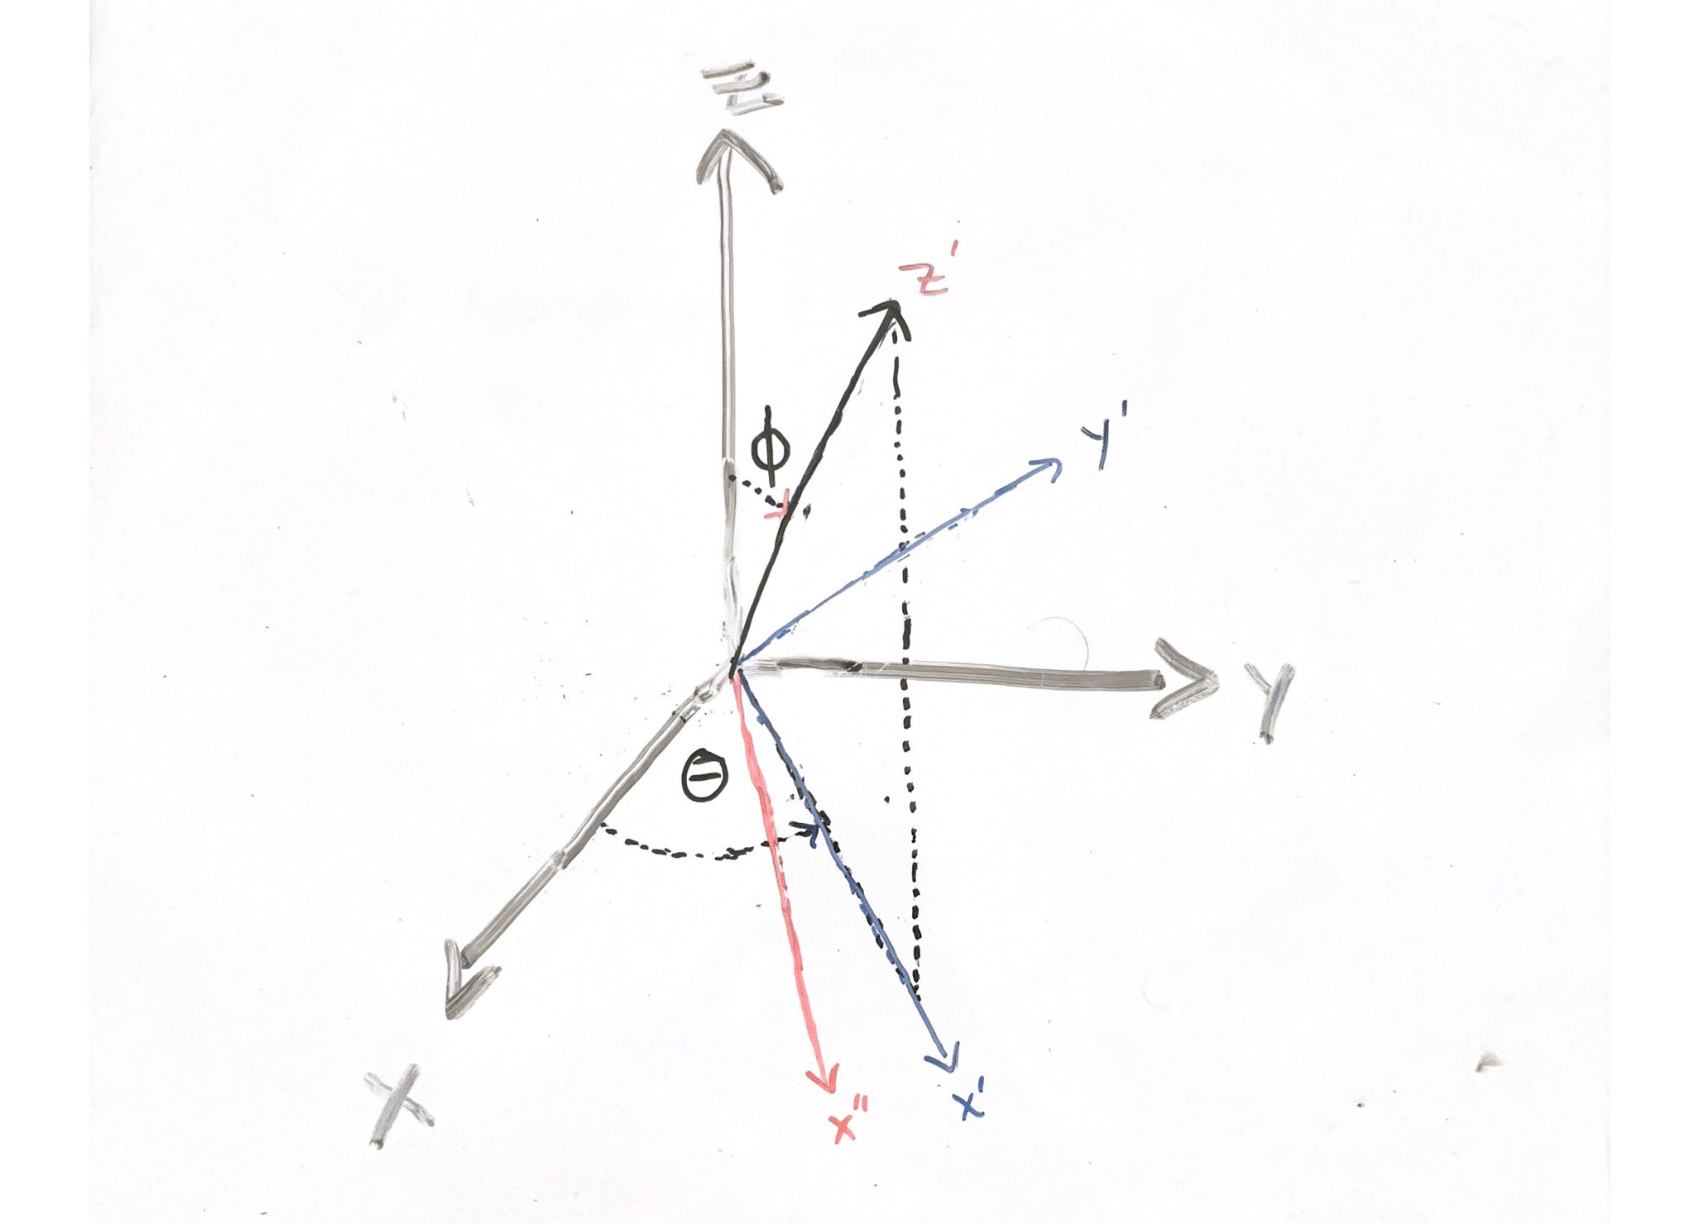
\includegraphics[width=0.7\textwidth]{pushzton}
	\caption{Rotation of the $z$-axis onto $n$}
\end{figure}

Using (3.8) and the above matrix, we can establish a relationship between $J_z$ and $J_n$. For any angle of rotation, $\psi$,

\begin{equation}
	\begin{aligned}
		e^{i\psi J_n} \\
							&= R_n(\psi)	\\
							&=R(\theta,\phi,0)R_z(\psi)R(\theta,\phi,0)^{-1}\\
							&=R(\theta,\phi,0) e^{i\psi J_z} R(\theta,\phi,0)^{-1}\\ 
							&= R(\theta,\phi,0) \sum_{n=0}^\infty \frac{(i\psi J_z)^n}{n!} R(\theta,\phi,0)^{-1} \\
							&= \sum_{n=0}^\infty \frac{(i\psi R(\theta,\phi,0)J_zR(\theta,\phi,0)^{-1})^n}{n!} \\
							&= e^{i\psi R(\theta,\phi,0)J_z R(\theta,\phi,0)^{-1}}\\
	\end{aligned}
\end{equation}

Comparing both sides of the equation, we can see that 

\begin{equation}
	\begin{aligned}
		J_n = R(\theta,\phi,0)J_z R(\theta,\phi,0)^{-1}
	\end{aligned}
\end{equation}

Further, arduous matrix algebra can be done explicitly to show the following identity holds: For any rotation matrix, $R$, and a specified generator, $J_k\in\{J_x,J_y,J_z\}$,

\begin{equation}
	\begin{aligned}
		RJ_kR^{-1} = J_x [R]_{1k} + J_y  [R]_{2k}  +J_z  [R]_{3k} 
	\end{aligned}
\end{equation}

Showing this is true consists of proving it for $R_z(\alpha)$ and $R_y(\beta)$ and arguing that any product of matrices of this form will also work. Combining (3.13) and (3.14), we get 

\begin{equation}
	\begin{aligned}
		J_n &= R(\theta,\phi,0)J_z R(\theta,\phi,0)^{-1} \\
			&= J_x * [R(\theta,\phi,0)]_{13} + J_y * [R(\theta,\phi,0)]_{23}  +J_z * [R(\theta,\phi,0)]_{33}\\
			 &= n_1J_x + n_2J_y + n_3J_z 
	\end{aligned}
\end{equation} 
\end{proof}

In this way, we can see that the generator of a rotation about any direction is a linear combination of the generators about our coordinate axes. For any generic rotation, $\psi$, about $n$, we see that 

\begin{equation}
	\begin{aligned}
		R_n(\psi) = e^{-i\psi n_1J_x}e^{-i\psi n_2J_y}e^{-i\psi n_3J_z}
	\end{aligned}
\end{equation} 

We can use this equation to write it in terms of a rotation's Euler angles in the following way:

\begin{equation}
	\begin{aligned}
		R(\alpha,\beta,\gamma) = e^{-i\alpha J_z}e^{-i\beta J_y}e^{-i\gamma J_z}
	\end{aligned}
\end{equation} 

In this sense, rotation in $\R^3$ can be written simply in terms of the angle measures and generators about coordinate axes.

\section{Irreducible Representations of $SO(3)$}

In order to uncover the irreducible representations of $SO(3)$, we will embark upon the same strategy that we used to find irreducible representations of $SO(2)$. Explicitly, we are looking to find invariant subspaces of our generator. However, we now have three generators to check, and the invariant subspace that we find has to coincide with every possible rotation built from the three. To add more complexity to this matter, we no longer are in an abelian group, which makes our struggle greater for a few reasons. First, finding invariant subspaces under these generators will be dependent on the order in which we apply the rotations. Secondly, irreducible representations need not be degree one anymore. We need to find an invariant subspace that exists independent of any order of rotation and that works with all our generators that are spanned by possibly an infinite set of vectors.

First, let us tackle the problem of commuting. We begin with the following definition.

\begin{definition}
	The \textbf{commutator} of two matrices $A$ and $B$ is defined by to be 
$$[A,B]=AB-BA$$
\end{definition}

By definition, two operators/matrices commute if and only if their commutator is equal to $0$. With this in mind, we can expect the generators of our rotations to have the following nontrivial commutators.

\begin{theorem}
	Let $J_k,J_l \in \{J_x,J_y,J_z\}$. Consider the word $xyz$, and all 6 rearrangements of it (identifying each rearrangement with a permutation in $S_3$). Then 
$$[J_k , J_l] = \begin{cases}
					0 & \text{if }k = l \\
					isign(klm)J_m& \text{else}
					\end{cases}$$
where $m$ is the label of the remaining generator in $\{J_x,J_y,J_z\}$.
\end{theorem}

\noindent\begin{proof} These nine commutators can all be verified by direct calculation. In the case where $k=l$, $[J_k,J_k] = J_kJ_k - J_kJ_k = 0$. However, if $k\neq l$, the calculation is dependent on the choice for $k$ and $l$. We will illustrate one example, and the other five commutators can be verified to follow a similar pattern. Take $k=x$ and $l=y$, our word $klm=xyz$ which represents the trivial permutation. Therefore, $sign(xyz)=1$.

\begin{equation}
	\begin{aligned}
		[J_x,J_y] &= J_xJ_y - J_yJ_x \\
					&= \begin{bmatrix}
							0 & 0 & 0\\
							0 & 0 & -i\\
							0 & i & 0
						\end{bmatrix}
						 \begin{bmatrix}
							0 & 0 & i\\
							0 & 0 & 0\\
							-i & 0 & 0
						\end{bmatrix}
						-
						\begin{bmatrix}
							0 & 0 & i\\
							0 & 0 & 0\\
							-i & 0 & 0
						\end{bmatrix}
						 \begin{bmatrix}
							0 & 0 & 0\\
							0 & 0 & -i\\
							0 & i & 0
						\end{bmatrix}\\
					&=  \begin{bmatrix}
							0 & 0 & 0\\
							-1 & 0 & 0\\
							0 & 0 & 0
						\end{bmatrix}
						-
						 \begin{bmatrix}
							0 & -1 & 0\\
							0 & 0 & 0\\
							0 & 0 & 0
						\end{bmatrix} \\
					&= \begin{bmatrix}
							0 & 1 & 0\\
							-1 & 0 & 0\\
							0 & 0 & 0
						\end{bmatrix} \\
					&=i \begin{bmatrix}
							0 & -i & 0\\
							i & 0 & 0\\
							0 & 0 & 0
						\end{bmatrix} \\
					&= i*sign(xyz)*J_z\\
	\end{aligned}
\end{equation} 

Clearly, transposing $x$ and $y$ will make the commutator negative (applying a transposition to $x$ and $y$ turns the word into $yxz$, so this is kept track of in the sign term). The other four cases can be recovered in a similar way. \end{proof}

While we can clearly see that these relationships give us a non-commutative structure, we can still glean some value from these commutators if we use them in a different context.

\begin{definition}
	A \textbf{Lie Algebra} is a vector space, $\mathfrak{g}$, together with a bilinear operation, $[\dot,\dot]$ that satisfies the the following identities:
\begin{itemize}
	\item$ [x,x] = 0$  $\forall x\in\mathfrak{g}$
	\item $[x,[y,z]] + [y,[z,x]] + [z[y,x]]= 0 $ $\forall x,y,z\in\mathfrak{g}$
\end{itemize}
\end{definition}

If we consider the commutator operation our bilinear operation, we can construct a Lie algebra (using standard addition and scalar multiplication of matrices). Keeping the generators $\{J_x,J_y,J_z\}$, we will denote this Lie algebra as $\mathfrak{so}(3) := \{a_1J_x + a_2J_y + a_3Jz \mid a_1,a_2,a_3\in\C\}$ We can see that any arbitrary element, $M\in \mathfrak{so}(3)$ takes the following form:

\begin{equation}
	\begin{aligned}
		M=i\begin{bmatrix}
		0 & -a_3 & a_2 \\
		 a_3 & 0 & -a_1\\
		-a_2 & a_1 & 0
		\end{bmatrix}
	\end{aligned}
\end{equation} 

showing us that there is a one-to-one correspondence between the skew-symmetric matrices of size $3\times 3$ and matrices in $\mathfrak{so}(3)$. With this in mind, we can make the argument that any representation of this Lie algebra ($\mathfrak{so}(3)$) will provide us with a representation of the Lie group ($SO(3)$). There is a deep reason for this connection that can be explored in the following source \cite{Hall}. The process for this is much the same as embarked upon for $SO(2)$, but since those representations were one-dimensional and revolved only around one generator, it was not necessary to introduce the complexity of Lie algebras just yet to create the representations. 

As we search for the representations of $\mathfrak{so}(3)$, we still need to find commuting generators. For the moment, it seems that we did not reduce our problem whatsoever, but rather added a layer of abstraction. In light of this, we can add even more abstraction to eventually shed some clarity on our circumstances.

\begin{definition}
	The \textbf{universal enveloping algebra} of a Lie algebra is the largest embedding of Lie algebra into an algebra. 
\end{definition}

The inherent utility of the universal enveloping algebra (of a Lie algebra) is that it is the most generic algebra that preserves the commutating properties of the Lie algebra. We will later discuss the necessity of appealing to this larger structure, but we will discuss what this space actually looks like. 

The construction of the universal enveloping algebra of $\mathfrak{so}(3)$ (which we will denote $A_{\mathfrak{so}(3)}$) follows this prototypical scheme: First, we construct the tensor algebra of $\mathfrak{so}(3)$. This takes the following form:

\begin{equation}
	\begin{aligned}
		T(\mathfrak{so}(3)) = \bigoplus_{i=0}^\infty \left(\bigotimes_{k=0}^i \mathfrak{so}(3)\right) = \left(\C\right) \oplus \left(\mathfrak{so}(3)\right) \oplus \left(\mathfrak{so}(3)\otimes \mathfrak{so}(3)\right) \oplus \hdots
	\end{aligned}
\end{equation} 

Now that we have created (free) tensor algebra on elements of $\mathfrak{so}(3)$, we can establish the commutation relations on elements. We identify each of our generators $J_i$ with its counterpart in the tensor algebra, $\mathfrak{J}_i$. We can construct an ideal, $I$ to be generated by the three elements defined below: 

$$\mathfrak{g_i} \coloneq \mathfrak{J}_k \otimes \mathfrak{J}_l - \mathfrak{J}_l\otimes \mathfrak{J}_k - \begin{cases}
	0 & \text{if }k=l	\\
	i*sign(klm) \mathfrak{J}_m &\text{else}
\end{cases}$$

We then gather our universal enveloping algebra on $\mathfrak{so}(3)$ by taking the corresponding quotient space.

$$A_{\mathfrak{so}(3)} \coloneq T(\mathfrak{so}(3)) / I$$

As of now, we have shifted our problem to looking for commutative elements in $A_{\mathfrak{so}(3)}$. What is the inherent significance of this? If we view our generators $J_x$, $J_y$, $J_z$ as elements in $A_{\mathfrak{so}(3)}$, we can see that the commutator relations are still satisfied as they are in $\mathfrak{so}(3)$. However, due to the construction, there is no way to meaningfully combine them. All that we know is that any formal combination of our generators can potentially be simplified with our commutator relations, and no other information is given. So, we must set out to find an element in $A_{\mathfrak{so}(3)}$ that commutes with all other elements.

\begin{definition}
	A \textbf{Casimir element} of a Lie algebra, $A$, is any element in the center of the universal enveloping algebra of $A$.
\end{definition}

This process, while a seemingly daunting task, is easily solved by taking a well-known physics concept to do the work for us. We define the element $\mathfrak{J^2} \coloneq (\mathfrak{J}_x \otimes \mathfrak{J}_x) \oplus (\mathfrak{J}_y \otimes \mathfrak{J}_y) \oplus (\mathfrak{J}_z \otimes \mathfrak{J}_z) = \mathfrak{J}_x^2 + \mathfrak{J}_y^2 + \mathfrak{J}_z^2$ where we suppress the tensor algebra notation for easier readbility. (It can be intuitively understood that any element referenced in $\mathfrak{this}$ $\mathfrak{script}$ will be contained in $A_{\mathfrak{so}(3)}$ and abide by its properties of multiplication).

\begin{theorem}
	$\mathfrak{J^2}$ is a Casimir element.
\end{theorem}

\noindent \begin{proof} Let $k\in \{x,y,z\}$.
\begin{equation}
\begin{aligned}
	[\mathfrak{J^2}, \mathfrak{J}_k] &= [\mathfrak{J}_x^2, \mathfrak{J}_k] + [\mathfrak{J}_y^2, \mathfrak{J}_k] + [\mathfrak{J}_z^2, \mathfrak{J}_k]\\
										 &=\sum_{\substack{m\in\{x,y,z\} \\ m\neq k}} \mathfrak{J}_m [\mathfrak{J}_m, \mathfrak{J}_k] + [\mathfrak{J}_m, \mathfrak{J}_k]\mathfrak{J}_m\\
										&= \mathfrak{J}_{m_1}(i\mathfrak{J}_{l_1})+ (i\mathfrak{J}_{l_1}) \mathfrak{J}_{m_1} + \mathfrak{J}_{m_2}(-i\mathfrak{J}_{l_2}) +(-i\mathfrak{J}_{l_2}) \mathfrak{J}_{m_2} \\
										&= 0
\end{aligned}
\end{equation}
where the last equality is established by the fact that our choice is limited to $m_2$ and $l_2$ are forced to be exactly $l_1$ and $m_1$ respectively. \end{proof}

The natural question to ask is why did we have to build the structure of the universal enveloping algebra to be able to use a seemingly straightforward element. The answer comes from the fact that there is no corresponding $J^2$ element in the Lie algebra $\mathfrak{so}(3)$. A direct computation would show us that:

\begin{equation} 
	\begin{aligned}
		J^2  &= J_x^2 + J_y^2 + J_z^2 \\
					&= \begin{bmatrix}
								0& 0 & 0 \\
								0 & 0 & -i \\
								0 & i & 0
							\end{bmatrix}^2 +\begin{bmatrix}
													0 & 0 & i \\
													0 & 0 & 0 \\
													-i & 0 & 0
												\end{bmatrix}^2 + \begin{bmatrix}
																			0 & -i & 0\\
																			i & 0 & 0 \\
																			0 & 0 & 0
																		\end{bmatrix}^2 \\
					&= \begin{bmatrix}
								0& 0 & 0 \\
								0 & 1 & 0 \\
								0 & 0 & 1
							\end{bmatrix} +\begin{bmatrix}
													1 & 0 & 0 \\
													0 & 0 & 0 \\
													0 & 0 & 1
												\end{bmatrix} + \begin{bmatrix}
																			1 & 0 & 0\\
																			0 & 1 & 0 \\
																			0 & 0 & 0
																		\end{bmatrix} \\
					&= \begin{bmatrix}
								2& 0 & 0 \\
								0 & 2 & 0 \\
								0 & 0 & 2
							\end{bmatrix} \\
					&= 2I_3 \notin \mathfrak{so}(3)
	\end{aligned}
\end{equation} 

Therefore, our discussion must be specific to $A_{\mathfrak{so}(3)}$ in order for us to develop any useful insight with commutative elements.

Letting $\phi$ be any irreducible representation of $A_{\mathfrak{so}(3)}$, the commutativity of $\mathfrak{J^2}$ shows us that for any $\mathfrak{J}_n \in A_{\mathfrak{so}(3)}$, $\phi(\mathfrak{J}_n)\phi(\mathfrak{J^2}) = \phi(\mathfrak{J^2})\phi(\mathfrak{J}_n)$. Schur's Theorem asserts that $\phi(\mathfrak{J^2}) = \lambda I_m$ where $\lambda\in\C$ and $m$ is the degree of the representation. This means that for any $v\in V$ (on which the representations are defined to be operators), $v$ is an eigenvector of $\phi(\mathfrak{J^2})$ with eigenvalue $\lambda$.

In search of our invariant subspace, we now must choose an eigenbasis of $V$ with respect to a basis of commuting generators (whose span collects all possible generators in $A_{\mathfrak{so}(3)}$). We can easily select $\mathfrak{J^2}$ and an additional generator from our typical collection $\{\mathfrak{J}_x,\mathfrak{J}_y,\mathfrak{J}_z\}$, but after choosing one, we can't choose any of the remaining options for fear of not commuting. Conventionally, we select $\{\mathfrak{J^2},\mathfrak{J}_z\}$ as our generators, and choose an eigenbasis of $V$ to be defined with respect to both these generators. With the remaining two generators, we construct two useful linear combinations that will aid us in our efforts.

\begin{equation}
	\begin{aligned}
		\mathfrak{J}_\pm = \mathfrak{J}_x \pm i\mathfrak{J}_y
	\end{aligned}
\end{equation} 

$\mathfrak{J}_+$ is referred to as the ``raising" generator and $\mathfrak{J}_-$ is referred to as the ``lowering generator". It is straightforward to verify that these new generators have special relationships with our conventionally selected generators as seen below:

\begin{equation}
	\begin{aligned}
		[\mathfrak{J}_z,\mathfrak{J}_+] = \mathfrak{J}_+
	\end{aligned}
\end{equation} 
\begin{equation}
	\begin{aligned}
		[\mathfrak{J}_z,\mathfrak{J}_-] = -\mathfrak{J}_-
	\end{aligned}
\end{equation} 
\begin{equation}
	\begin{aligned}
		[\mathfrak{J}_+,\mathfrak{J}_-] = 2\mathfrak{J}_z
	\end{aligned}
\end{equation} 
\begin{equation}
	\begin{aligned}
		\mathfrak{J}^2 = (\mathfrak{J}_z)^2  -\mathfrak{J}_z +\mathfrak{J}_+\mathfrak{J}_- = (\mathfrak{J}_z)^2 +\mathfrak{J}_z+ \mathfrak{J}_-\mathfrak{J}_+
	\end{aligned}
\end{equation} 
\begin{equation}
	\begin{aligned}
		\phi_{\mathfrak{J}_\pm}^\dag = \phi_{\mathfrak{J}_\mp}
	\end{aligned}
\end{equation} 

Using these identities, one can see that for any eigenvector, $v_m$, corresponding to the generator $J_z$ with eigenvalue $m$, then the following two identities hold:

\begin{equation}
	\begin{aligned}
		\phi_{\mathfrak{J}_z\mathfrak{J}_+}(v_m) &= \phi_{\mathfrak{J}_z\mathfrak{J}_+ (-\mathfrak{J}_+\mathfrak{J}_z + \mathfrak{J}_+\mathfrak{J}_z)}(v_m) \\
					&= \phi_{[\mathfrak{J}_z,\mathfrak{J}_+]}(v_m) + \phi_{\mathfrak{J}_+\mathfrak{J}_z}(v_m) \\
					&= \phi_{\mathfrak{J}_+}(v_m) + \phi_{\mathfrak{J}_+\mathfrak{J}_z}(v_m) \\
					&= \phi_{\mathfrak{J}_+(I + \mathfrak{J}_z)}(v_m) \\					
					&= \phi_{\mathfrak{J}_+}((\phi_{I} + \phi_{\mathfrak{J}_z})(v_m)) \\
					&= \phi_{\mathfrak{J}_+}  ((1+m)v_m) \\
					&= (m + 1)\phi_{J_+}(v_m)
	\end{aligned}
\end{equation} 
\begin{equation}
	\begin{aligned}
		\phi_{\mathfrak{J}_z\mathfrak{J}_-}(v_m) &= \phi_{\mathfrak{J}_z\mathfrak{J}_- (-\mathfrak{J}_-\mathfrak{J}_z + \mathfrak{J}_-\mathfrak{J}_z)}(v_m) \\
&=\phi_{[\mathfrak{J}_z,\mathfrak{J}_- ]}(v_m) + \phi_{\mathfrak{J}_-\mathfrak{J}_z}(v_m)\\
					&= \phi_{-\mathfrak{J}_-}(v_m) + \phi_{\mathfrak{J}_-\mathfrak{J}_z}(v_m)\\
					&= \phi_{\mathfrak{J}_-(-I + \mathfrak{J}_z)}(v_m) \\
					&= \phi_{\mathfrak{J}_-}((\phi_{-I} + \phi_{\mathfrak{J}_z})(v_m)) \\
					&= \phi_{\mathfrak{J}_-} ((-1+m)(v_m) \\
					&= (m - 1)\phi_{\mathfrak{J}_-}(v_m)\\
	\end{aligned}
\end{equation} 

These identities give an explicit reason for the naming convention (the raising generator increases the eigenvalue by $1$ and the lowering generator decreases it by $1$). With this, we conclude that repeated applications of $\phi_{\mathfrak{J}_+}$ or $\phi_{\mathfrak{J}_-}$ give us new eigenvectors of $\phi_{\mathfrak{J}_z}$, corresponding to eigenvalues $m + k$ and $m-l$ where $k$ represents the number of repeated applications of $\phi_{\mathfrak{J}_+}$ and $l$ represents the number of repeated applications of $\phi_{\mathfrak{J}_-}$ respectively. We can only repeat this process a finite number of times, as we are working in a finite-dimensional vector space. Let us shift our focus somewhat to consider $k$ to be the maximum number of applications of $\phi_{\mathfrak{J}_+}$ before $\phi_{\mathfrak{J}_+}^{k+1}(v_k) = 0$. Let $\lambda$ be the eigenvalue corresponding to eigenvector $\phi_{\mathfrak{J}_+}^{k}(v_{k-1})$ of the operator $\phi_{\mathfrak{J}_z}$. Then, 

\begin{equation}
	\begin{aligned}
		\phi_{\mathfrak{J^2}}\phi_{\mathfrak{J}_+}^k(v_{k-1}) = \phi_{(\mathfrak{J}_z)^2 +\mathfrak{J}_z+ \mathfrak{J}_-\mathfrak{J}_+}(\phi_{\mathfrak{J}_+}^k(v_{k-1})) = \lambda(\lambda + 1) \phi_{J_+}^kv_{k-1}
	\end{aligned}
\end{equation} 

Since $\phi_{\mathfrak{J^2}}$ is a multiple of the identity, it must be the case that $\lambda(\lambda +1)$ is the only eigenvalue of $\phi_{\mathfrak{J^2}}$. Further, repeated applications of $\phi_{\mathfrak{J}_-}$ will decrease the eigenvalue of $\phi_{\mathfrak{J}_z}$ by $1$ for each application. However, this can only happen a finite number of times before we terminate. Therefore, if $l$ is the last application number of applications before  $\phi_{\mathfrak{J}_-}^{l+1}(v_{l}) = 0$ and $\phi_{J_z}v_l = l$.
\begin{equation}
	\begin{aligned}
		0 &= v_{l}  \phi_{\mathfrak{J}_-}^\dag \phi_{\mathfrak{J}_-} v_{l} \\
		&= v_{l} \phi_{\mathfrak{J}_+}\phi_{\mathfrak{J}_-}v_{l} \\
			&= v_{l}\phi_{\mathfrak{J^2} - (\mathfrak{J}_z)^2 + \mathfrak{J}_z}v_{l} \\
		&= \lambda(\lambda+ 1) - l(l - 1)\\
	\end{aligned}
\end{equation} 

Which implies that $\lambda = -l$. Given that we arrived at eigenvalue $l$ from $\lambda$ by applying the lowering operator an integer number of times, $\lambda - l \in \Z^+ \implies 2\lambda\in\Z^+ \implies \lambda = \frac{n}{2}$ for some $n\in\Z^+.$


\begin{theorem}
	The irreducible representations of the $A_{\mathfrak{so}(3)}$ are characterized by eigenvalues that take on positive integer and positive half-integer values. If $\lambda$ is one such eigenvalue, then we can construct our eigenvectors, $\{v_m\}_{m=-\lambda}^\lambda$, corresponding to $\phi_{\mathfrak{J}_z}$ with eigenvalue $m$, using the raising or lowering operators. This gives us a degree $2\lambda +1$ representation characterized by the following relationships:
$$\phi_{\mathfrak{J}^2}(v_m) = \lambda(\lambda+1)v_m$$
$$\phi_{\mathfrak{J}_z}(v_m) =  mv_m$$ 
$$v_{m+1} =  \frac{\phi_{\mathfrak{J}_\pm}(v_m)}{\sqrt{\lambda(\lambda+1) - m(m\pm 1)}}$$
\end{theorem}
\noindent where the normalizing factor comes from a brief calculation similar to the matrix product calculation done in (3.32). Theorem (3.10) gives us a way to calculate an irreducible, unitary representation up to any degree. The unitary aspect comes from the fact that $\{v_m\}$ are normalized and orthogonal by their construction. When we do the calculations, we have constructed our operators (in the image of our representation) and seek to construct an orthonormal basis with respect to these operators. As we have shown, following this form will ensure that we cannot create a nontrivial-invariant subspace, due to the fact that the cyclical nature of our eigenbasis construction. Explicitly, every vector in this basis will be an eigenvector of $\phi_{\mathfrak{J^2}}$, and since this operator commutes with every other, we inherit a set of eigenvectors that will span the entire space.

Given our hard work to establish a representation on $A_{\mathfrak{so}(3)}$, we can immediately conclude that we can construct a representation on $SO(3)$. Any rotation under the image of such an irreducible representation must behave in the following way:

\begin{equation}
\begin{aligned}
	\phi_j(R(\alpha,\beta,\gamma)) &= e^{-i\alpha\phi_{\mathfrak{J}_z}}e^{-i\beta\phi_{\mathfrak{J}_y}}e^{-i\gamma\phi_{\mathfrak{J}_z}}	
\end{aligned}
\end{equation}

We are required to compute explicitly $\phi_{\mathfrak{J}_z}$ and $\phi_{\mathfrak{J}_y}$ to make use of these formulas. The following example will illustrate this process more closely.

\begin{example}\end{example}
	Take $\lambda= \frac{1}{2}$. We expect the degree of our representation to be $2$ and we can immediately conclude that:

\begin{equation}
\begin{aligned}
	\phi_{\mathfrak{J^2}} = \begin{bmatrix}
									\frac{3}{4} & 0 \\
									0 & \frac{3}{4}
								\end{bmatrix}
\end{aligned}
\end{equation}
and 
\begin{equation}
\begin{aligned}
	\phi_{\mathfrak{J}_z} = \begin{bmatrix}
									\frac{1}{2} & 0 \\
									0 & \frac{-1}{2}
								\end{bmatrix}
\end{aligned}
\end{equation}

Using the identities found in (3.24-3.28), we can calculate $\phi_{\mathfrak{J}_\pm}$ as 

\begin{equation}
\begin{aligned}
	\phi_{\mathfrak{J}_+} = \begin{bmatrix}
									0 & 1 \\
									0 & 0
								\end{bmatrix}
\end{aligned}
\end{equation}
\begin{equation}
\begin{aligned}
	\phi_{\mathfrak{J}_-} = \begin{bmatrix}
									0 & 0 \\
									1 & 0
								\end{bmatrix}
\end{aligned}
\end{equation}
We can use these two matrices to solve a system of equations to acquire $\phi_{\mathfrak{J}_y}$ and $\phi_{\mathfrak{J}_x}$.
\begin{equation}
\begin{aligned}
	\phi_{\mathfrak{J}_x} = \begin{bmatrix}
									0 & \frac{1}{2} \\
									\frac{1}{2} & 0
								\end{bmatrix}
\end{aligned}
\end{equation}
\begin{equation}
\begin{aligned}
	\phi_{\mathfrak{J}_y} = \begin{bmatrix}
									0 & \frac{1}{2i} \\
									\frac{-1}{2i} & 0
								\end{bmatrix}
\end{aligned}
\end{equation}

We note that $\phi_{\mathfrak{J}_z}$ and $\phi_{\mathfrak{J}_y}$ are a scalar multiple away from having the desirable property that its square is the identity. Therefore, any rotation under $\phi$ is represented by the matrix

\begin{equation}
\begin{aligned}
	&\phi_\frac{1}{2}(R(\alpha,\beta,\gamma)) \\
	&= e^{-i\alpha\phi_{\mathfrak{J}_z}}e^{-i\beta\phi_{\mathfrak{J}_y}}e^{-i\gamma\phi_{\mathfrak{J}_z}}	\\
	&= (\cos(\frac{\alpha}{2})I_2 -i\sin(\frac{\alpha}{2})2*\phi_{\mathfrak{J}_z})(\cos(\frac{\beta}{2})I_2 -i\sin(\frac{\beta}{2})\phi_{\mathfrak{J}_y})(\cos(\frac{\gamma}{2})I_2 -i\sin(\frac{\gamma}{2})\phi_{\mathfrak{J}_z})\\
	&=\begin{small}\begin{bmatrix}
			\cos(\frac{\alpha}{2}) - i (\sin(\frac{\alpha}{2}) & 0\\
			0 & \cos(\frac{\alpha}{2}) + i (\sin(\frac{\alpha}{2})
		\end{bmatrix}
		\begin{bmatrix}
			\cos(\frac{\beta}{2}) & -\sin(\frac{\beta}{2}) \\
			  \sin(\frac{\beta}{2}) & \cos(\frac{\beta}{2}) 
		\end{bmatrix}
\begin{bmatrix}
			\cos(\frac{\gamma}{2}) - i (\sin(\frac{\gamma}{2}) & 0\\
			0 & \cos(\frac{\gamma}{2}) + i (\sin(\frac{\gamma}{2})
		\end{bmatrix}\end{small} \\
		&=\begin{bmatrix}
			e^{-i\frac{\alpha}{2}}\cos(\frac{\beta}{2})e^{-i\frac{\gamma}{2}} & -e^{-i\frac{\alpha}{2}}\sin(\frac{\beta}{2})e^{-i\frac{\gamma}{2}} \\
			e^{-i\frac{\alpha}{2}}  \sin(\frac{\beta}{2})e^{-i\frac{\gamma}{2}} & e^{-i\frac{\alpha}{2}}\cos(\frac{\beta}{2}) e^{-i\frac{\gamma}{2}}
		\end{bmatrix}
\end{aligned}
\end{equation}

It is worth noting that this example illustrates a multi-valued representation, seeing as $\phi_\frac{1}{2}(R(0,2\pi,0)) = -I_2$. In general, all of the half-integer eigenvalue representations will behave in this way.